\section{Introduction}

In this chapter, we will focus on the \textit{parser}, which is the part of our project that reads the input sequence given by the preprocessor alongside context information and outputs a so-called \verb|FormattedResponse|. 

It is written in Python and relies heavily on the Lark library.

The parser recursively works its way through the \verb|Tree| object given by Lark, and iteratively builds up the script, brackets, and options for its output.

Figure~\ref{fig:parser-flowchart_full_combined} shows a flowchart diagram of the entire parser, where the parts that are discussed in this section are depicted in detail. 

\begin{figure}[H]
    \centering
    \begin{subfigure}[b]{\linewidth}
        \centering
        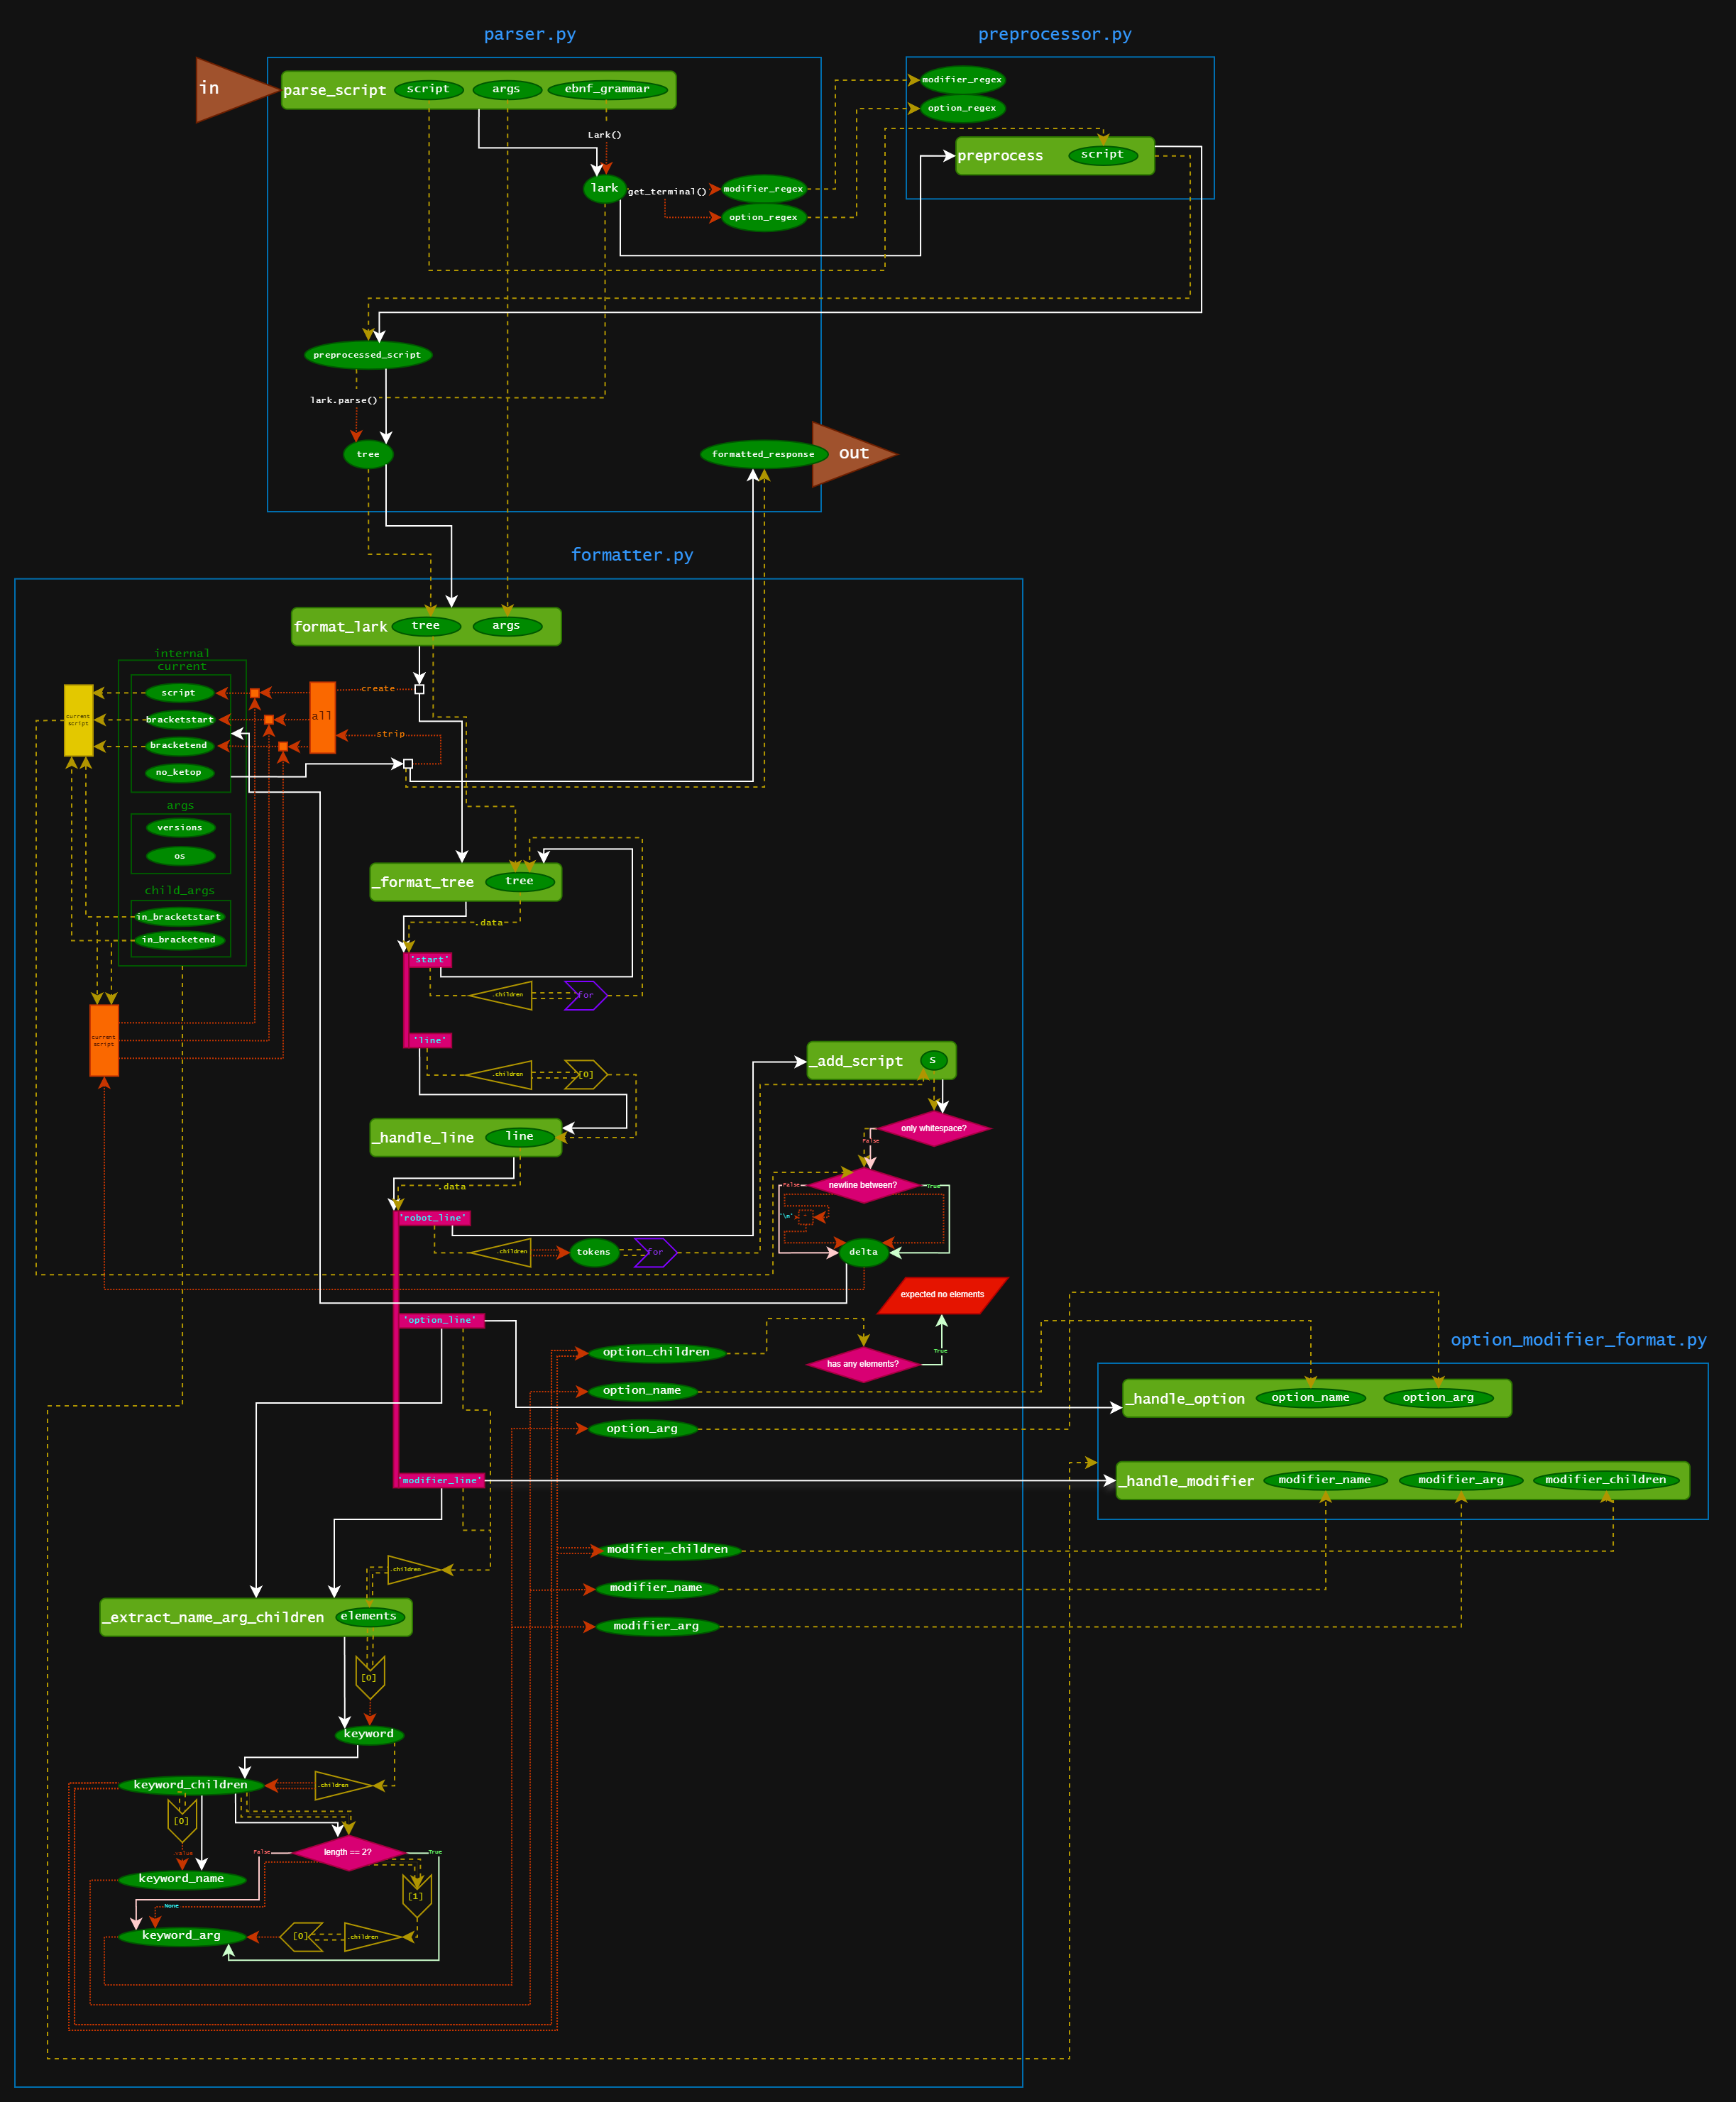
\includegraphics[width=0.35\linewidth]{pics/parser-flowchart/full.png}
        \caption{Downsized flowchart diagram of the parser.}
        \label{fig:parser-flowchart_full}
    \end{subfigure}\hfill
    \begin{subfigure}[b]{\linewidth}
        \centering
        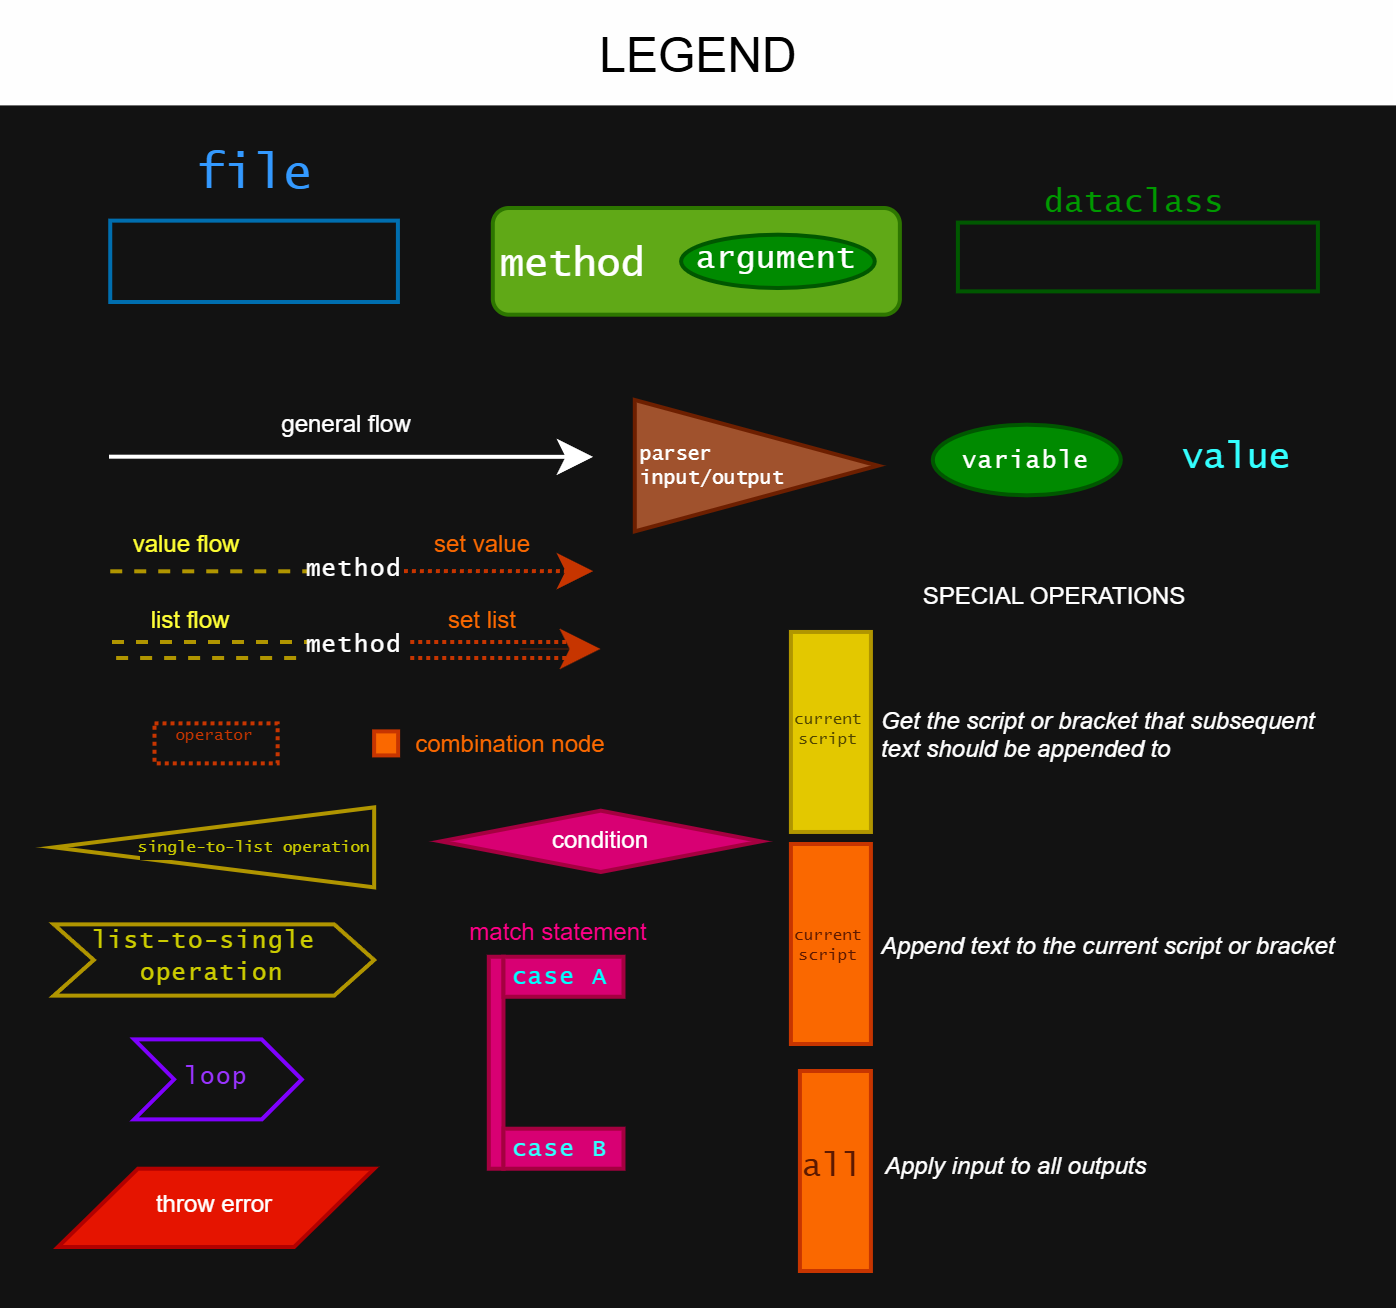
\includegraphics[width=0.6\linewidth]{pics/parser-flowchart/legend.png}
        \caption{Legend of the parser flowchart diagram.}
        \label{fig:parser-flowchart_legend}
    \end{subfigure}
    \caption{Full flowchart diagram of the parser with its legend.}
    \label{fig:parser-flowchart_full_combined}
\end{figure}

It is important to note that while Figure~\ref{fig:parser-flowchart_full} is at a size where it may not be possible to make out details, subsequent sections of this chapter include enlarged variants, as seen in Figures~\ref{fig:parser-flowchart_general_combined},~\ref{fig:parser-flowchart_line-formatting_combined},~\ref{fig:parser-flowchart_line-formatting_location}, and~\ref{fig:parser-flowchart_extract-name-arg-children_combined}.

\section{High-Level Overview}

In a nutshell, the parser takes an input in the form of a script as a string, a few contextual arguments as \verb|FormatterArgs|, and a Lark grammar, which resembles an EBNF grammar, as a string, and outputs a \verb|FormattedResponse|, as is evident by its method header:

\begin{lstlisting}[language=Python, caption={Method header of \texttt{parse\_script}.}, label={lst:method_header_parser_parse_script}]
def parse_script(script:str, args:FormatterArgs, ebnf_grammar:str)->FormattedResponse:
\end{lstlisting}

\subsection{Input: Script}

The script is the the raw Robot script that is to be parsed. Importantly, this input should not already have gone through the preprocessor step mentioned in Chapter~\ref{chap:preprocessor}, as it is done in the function.

\subsection{Input: Arguments}

In the method header, \verb|formatter_args| refers to an instance of the \verb|FormatterArgs| class, which is defined to be the following:

\begin{lstlisting}[language=Python, caption={Class definition of \texttt{FormatterArgs}.}, label={lst:class_definition_parser_formatter_args}]
@dataclass
class FormatterArgs:
    versions:dict[str, str] # label -> version
    os:str|None
\end{lstlisting}

This is used for providing the contextual input, which, in our case, is needed to evaluate the conditions specified in the \verb|@VERSION| and \verb|@OS| modifiers. 

Here, \verb|versions| should be a dictionary object that maps the label of a module to its actual version on the KeTop. In the actual implementation of \verb|@VERSION|, the operation specified in the argument will be checked against the version provided here for the respective module. 

\verb|os| refers to the operating system of the KeTop as a string, or \verb|None| if one is not provided or present (as is generally the case when, for instance, the \verb|no_ketop| flag is set). In the actual implementation of \verb|@OS|, the block body will only be included if the operating system specified in the argument equals the operating system provided here. If no operating system is provided, \verb|@OS| will always discard its block body.

\subsection{Input: Lark grammar}

The Lark grammar, in the method header labeled as \verb|ebnf_grammar|, represents ``a list of rules and terminals that together define a language''\cite{py-module-lark-grammar} as a string. While the Lark library uses its own syntax, it is based on EBNF~\cite{py-module-lark-grammar}.

In our project, the following string, which is a modified form of the our EBNF to abide by Lark's expected syntax, gets used:

\begin{lstlisting}[caption={Our EBNF defined using Lark's syntax.}, label={lst:our_ebnf_lark}]
start: N* (line N*)*

robot_line: /[^(@|\n)].+?(?=\n)/

option_line: "@" option 

modifier_line: "@" modifier ( N )* ( line N* )* "@" "END"

line: modifier_line | option_line | robot_line

modifier: ALLOWED_MODIFIERS arg?
option: ALLOWED_OPTIONS arg?

arg: /[ \t]+[^\n]*/

N: "\n"

%import common.WS_INLINE
%ignore WS_INLINE

ALLOWED_OPTIONS: "NO_KETOP" 
ALLOWED_MODIFIERS: "VERSION" | "BRACKETSTART" | "BRACKETEND" | "OS" | "PREAMBLE"
\end{lstlisting}

The following is changed in listing \ref{lst:our_ebnf_lark} compared to listing \ref{lst:our_ebnf}:
\begin{itemize}
    \item Grammar definition syntax is changed from \verb|=| to \verb|:| and the seperator character between terminals (\verb|,|) and the end-of-rule character (\verb|;|) are omitted.
    \item Repetition is changed from using curly braces (\verb|{...}|) to an asterisk (\verb|...*|). It is important to note that, while it is not needed for our EBNF, Lark also allows for the definition of \textit{one or more} using a plus sign (\verb|...+|) instead.
    \item Optionals are changed from using square brackets (\verb|[...]|) to \verb|...?|.
    \item \gls{regex} tokens are written using slashes (\verb|/.../|).
    \item Terminals (here \verb|N|, \verb|ALLOWED_OPTIONS|, and \verb|ALLOWED_MODIFIERS|) are defined using uppercase.
    \item The verbose definition of the \verb|block body| rule is omitted, and it is instead defined directly within a \verb|modifier_line|.
    \item Inline whitespace is being explicitely ignored using \verb|%import common.WS_INLINE| and \verb|%ignore common.WS_INLINE|. % it says there's an error here because of the percent sign, but it seems to work fine
\end{itemize}

It is important to mention that, while it might be possible to provide a different grammar, it is very likely to cause issues given the strict adherence of our parser to the above grammar. 

\subsection{Output: FormattedResponse}

As long as no exceptions occur, the output of the \verb|parse_script| function will be an instance of the \verb|FormattedResponse| class, which is defined to be the following:

\begin{lstlisting}[language=Python, caption={Class definition of \texttt{FormattedResponse}.}, label={lst:class_definition_parser_formatted_response}]
@dataclass
class FormattedResponse:
    script:str
    preamble_dict:dict[int, str]
    bracketstart:str
    bracketend:str
    no_ketop:bool 
\end{lstlisting}

Here, \verb|script| refers to the general part of the script that is not part of a \textit{bracket}. The term \textit{bracket} refers to a block body of either \verb|@PREAMBLE|, \verb|@BRACKETSTART|, or \verb|@BRACKETEND|. If a Robot script with no Script Assembler keywords is provided as input, aside from possible minor whitespace changes, it will be returned without edit in \verb|script|. 

\verb|preamble_dict| is a dictionary that maps the block bodies of \verb|@PREAMBLE| modifiers to the number given by their respective arguments. 

\verb|bracketstart| and \verb|bracketend| contain the block bodies of \verb|@BRACKETSTART| and\\
\verb|@BRACKETEND| respectively. 

\verb|no_ketop| represents whether or not the \verb|no_ketop| flag is enabled; i.e.\ whether or not the input script contains the \verb|@NO_KETOP| modifier.

\section{Lark}

Lark is a parsing library for Python which can parse any context-free grammar to an object known as a \textit{tree}~\cite{py-module-lark}.

After preprocessing, the Script Assembler uses the input script on Lark's \verb|parse| method to get a \verb|Tree| object which, amongst others, includes two important properties: \verb|data| and \verb|children|.

A \verb|Tree| object represents a rule with a name, for example, the outermost rule of a parsed script being \verb|"start"|, alongside, if present, its children, which, in the example of \verb|"start"| are \verb|"line"|s. A \textit{child} is commonly a \verb|Tree| as well, however it may also be a \verb|Token|~\cite{py-module-lark-api}.

According to Lark's official \gls{api} reference, a \verb|Token| is described as the following:

\begin{quote}
``A string with meta-information, that is produced by the lexer. When parsing text, the resulting chunks of the input that haven't been discarded, will end up in the tree as Token instances. The Token class inherits from Python's \verb|str|, so normal string comparisons and operations will work as expected.''\cite{py-module-lark-api}
\end{quote}

In our parser, we mainly work with \verb|Tree|s to differentiate between lines and keywords, and \verb|Token|s for the contents of robot lines and keyword arguments. 

\section{General Procedure}

The \verb|parse_script| starts by creating an instance of the \verb|Lark| class using the provided grammar. Using Lark's \verb|get_terminal| function, the allowed modifiers and options as specified in the grammar are fetched and, together with the input script, passed to the preprocessor. 

Afterwards, using Lark's \verb|parse| method, the preprocessed script is then converted to a \verb|Tree| object. This is passed to the \verb|format_lark| function, which utilizes the provided \verb|FormatterArgs| to turn it into a \verb|FormattedResponse|, which is then returned. 

Figure~\ref{fig:parser-flowchart_general_combined} highlights this procedure.

\begin{figure}[H]
    \centering
    
    \begin{subfigure}[b]{\linewidth}
        \centering
        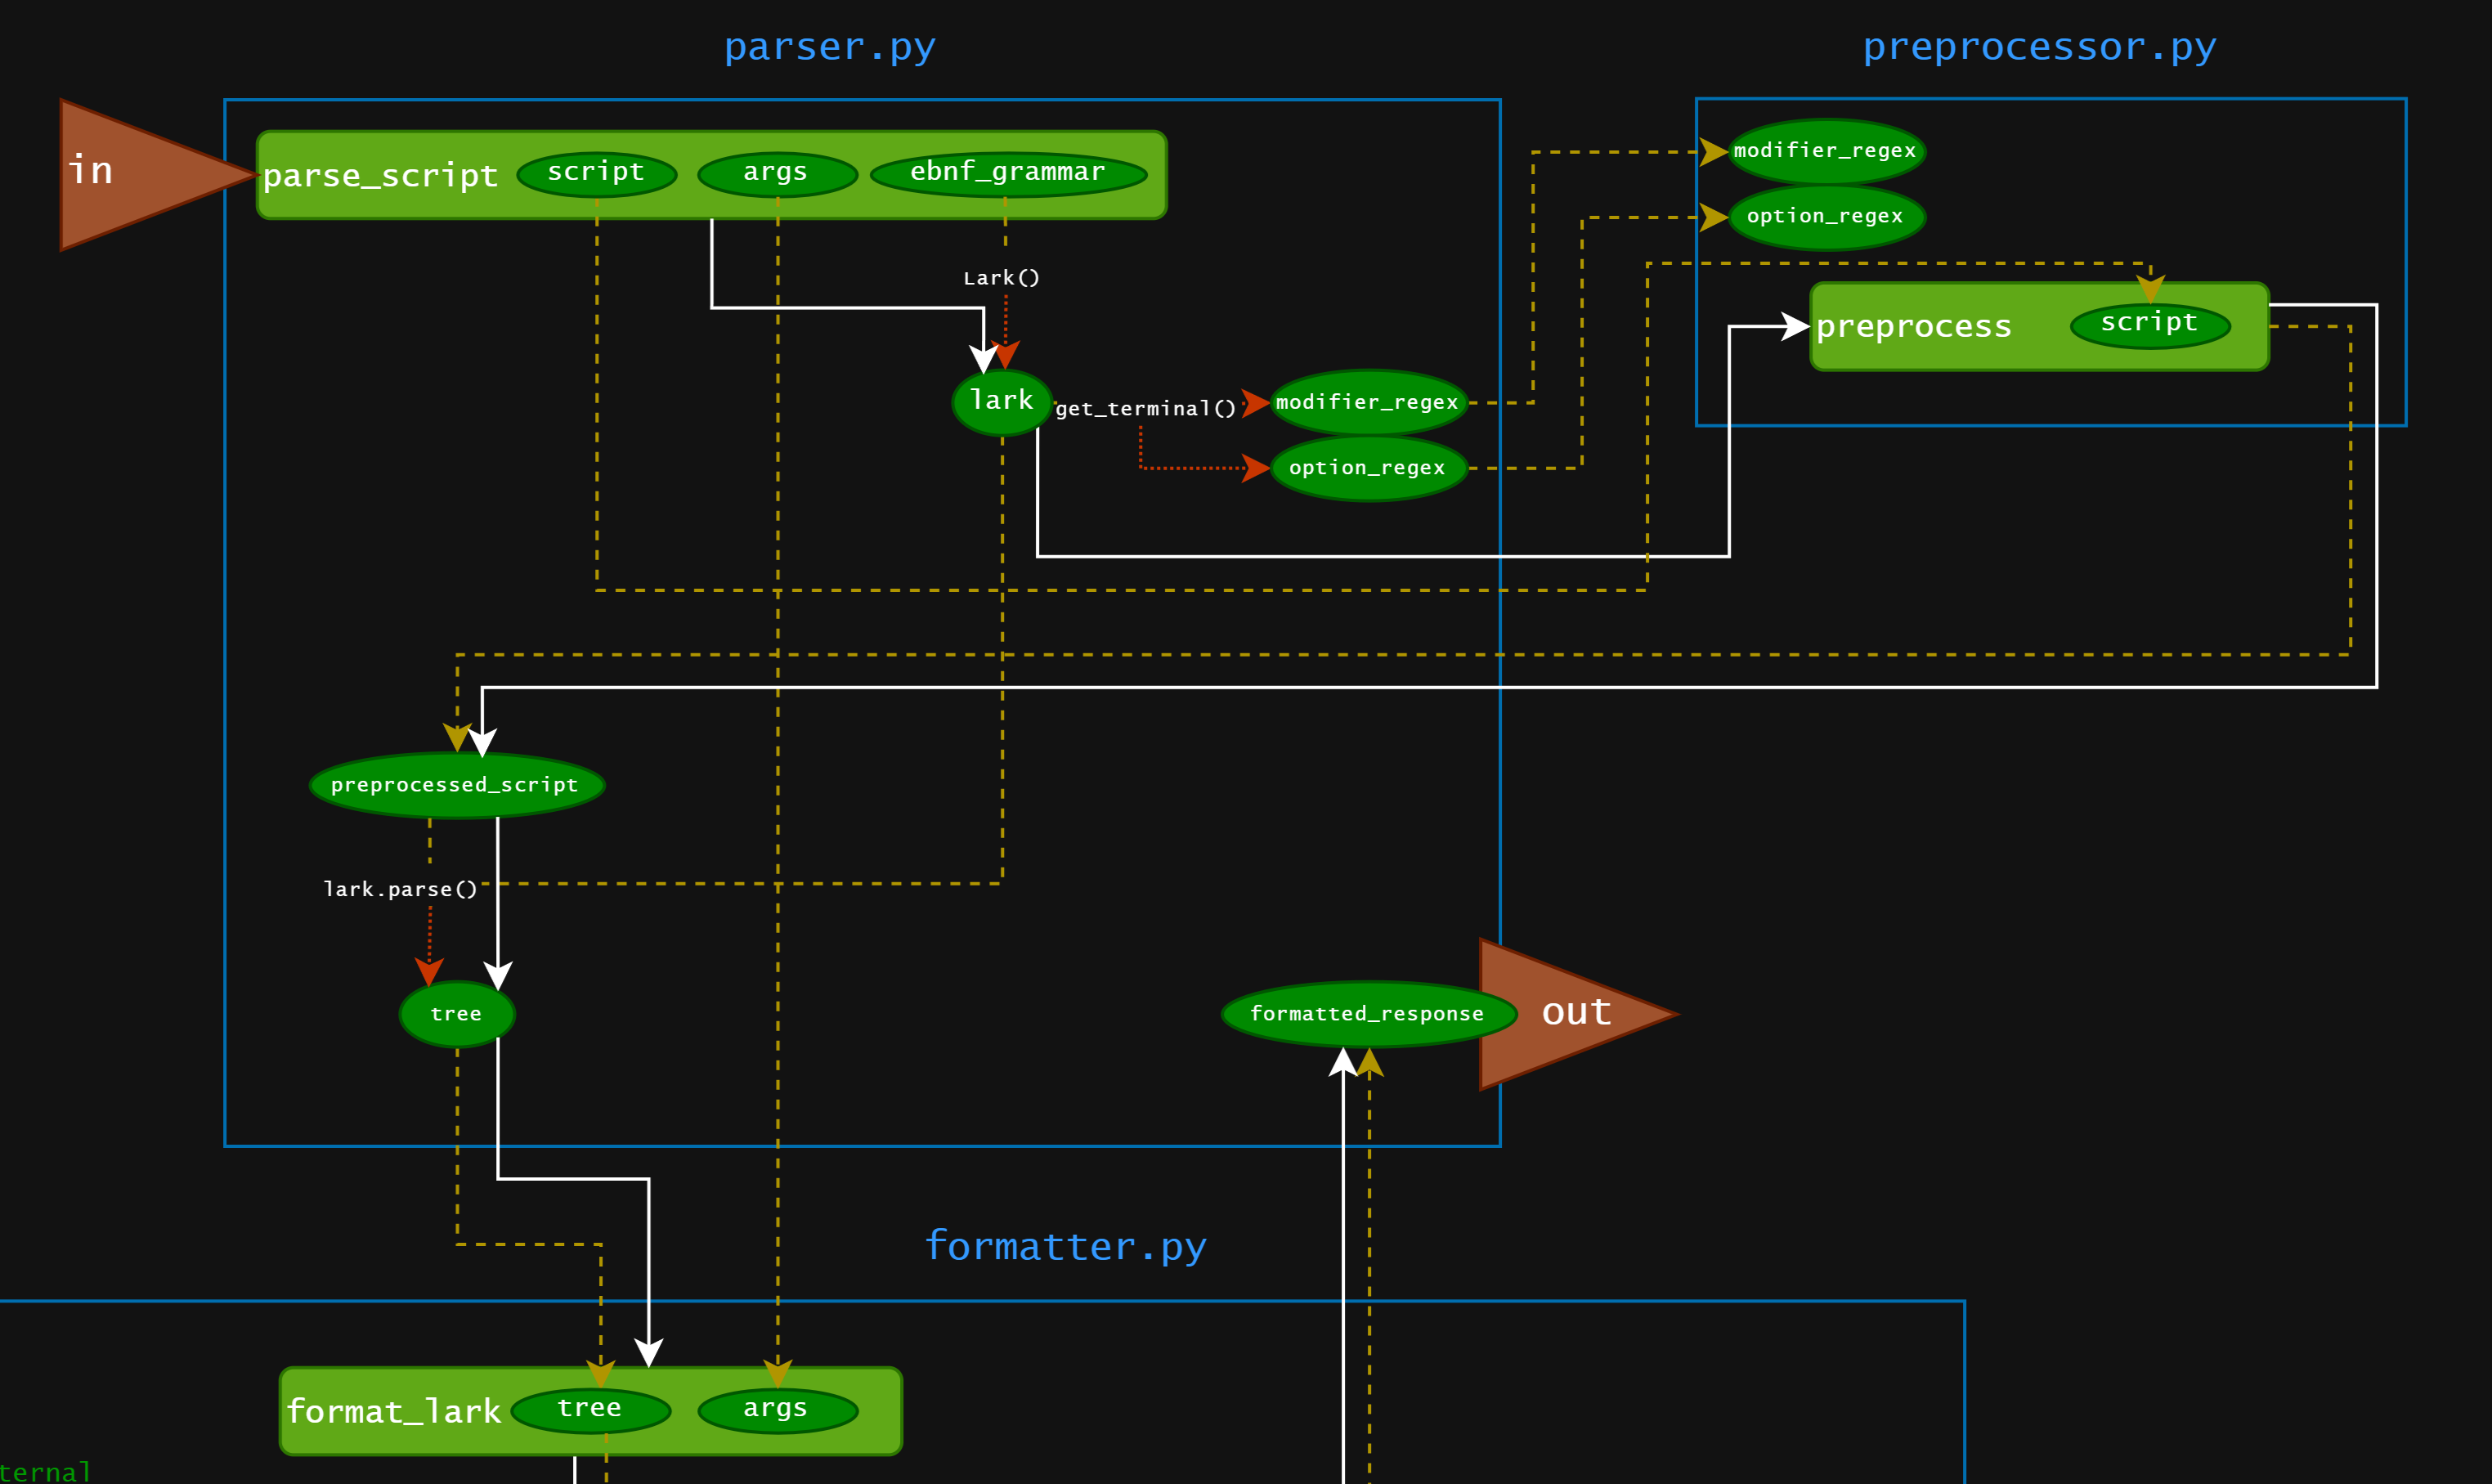
\includegraphics[width=\linewidth]{pics/parser-flowchart/general.png}
        \caption{The detailed part of the parser's flowchart diagram which illustrates the general procedure.}
        \label{fig:parser-flowchart_general}
    \end{subfigure}

    \vspace{6pt}

    \begin{subfigure}[b]{\linewidth}
        \centering
        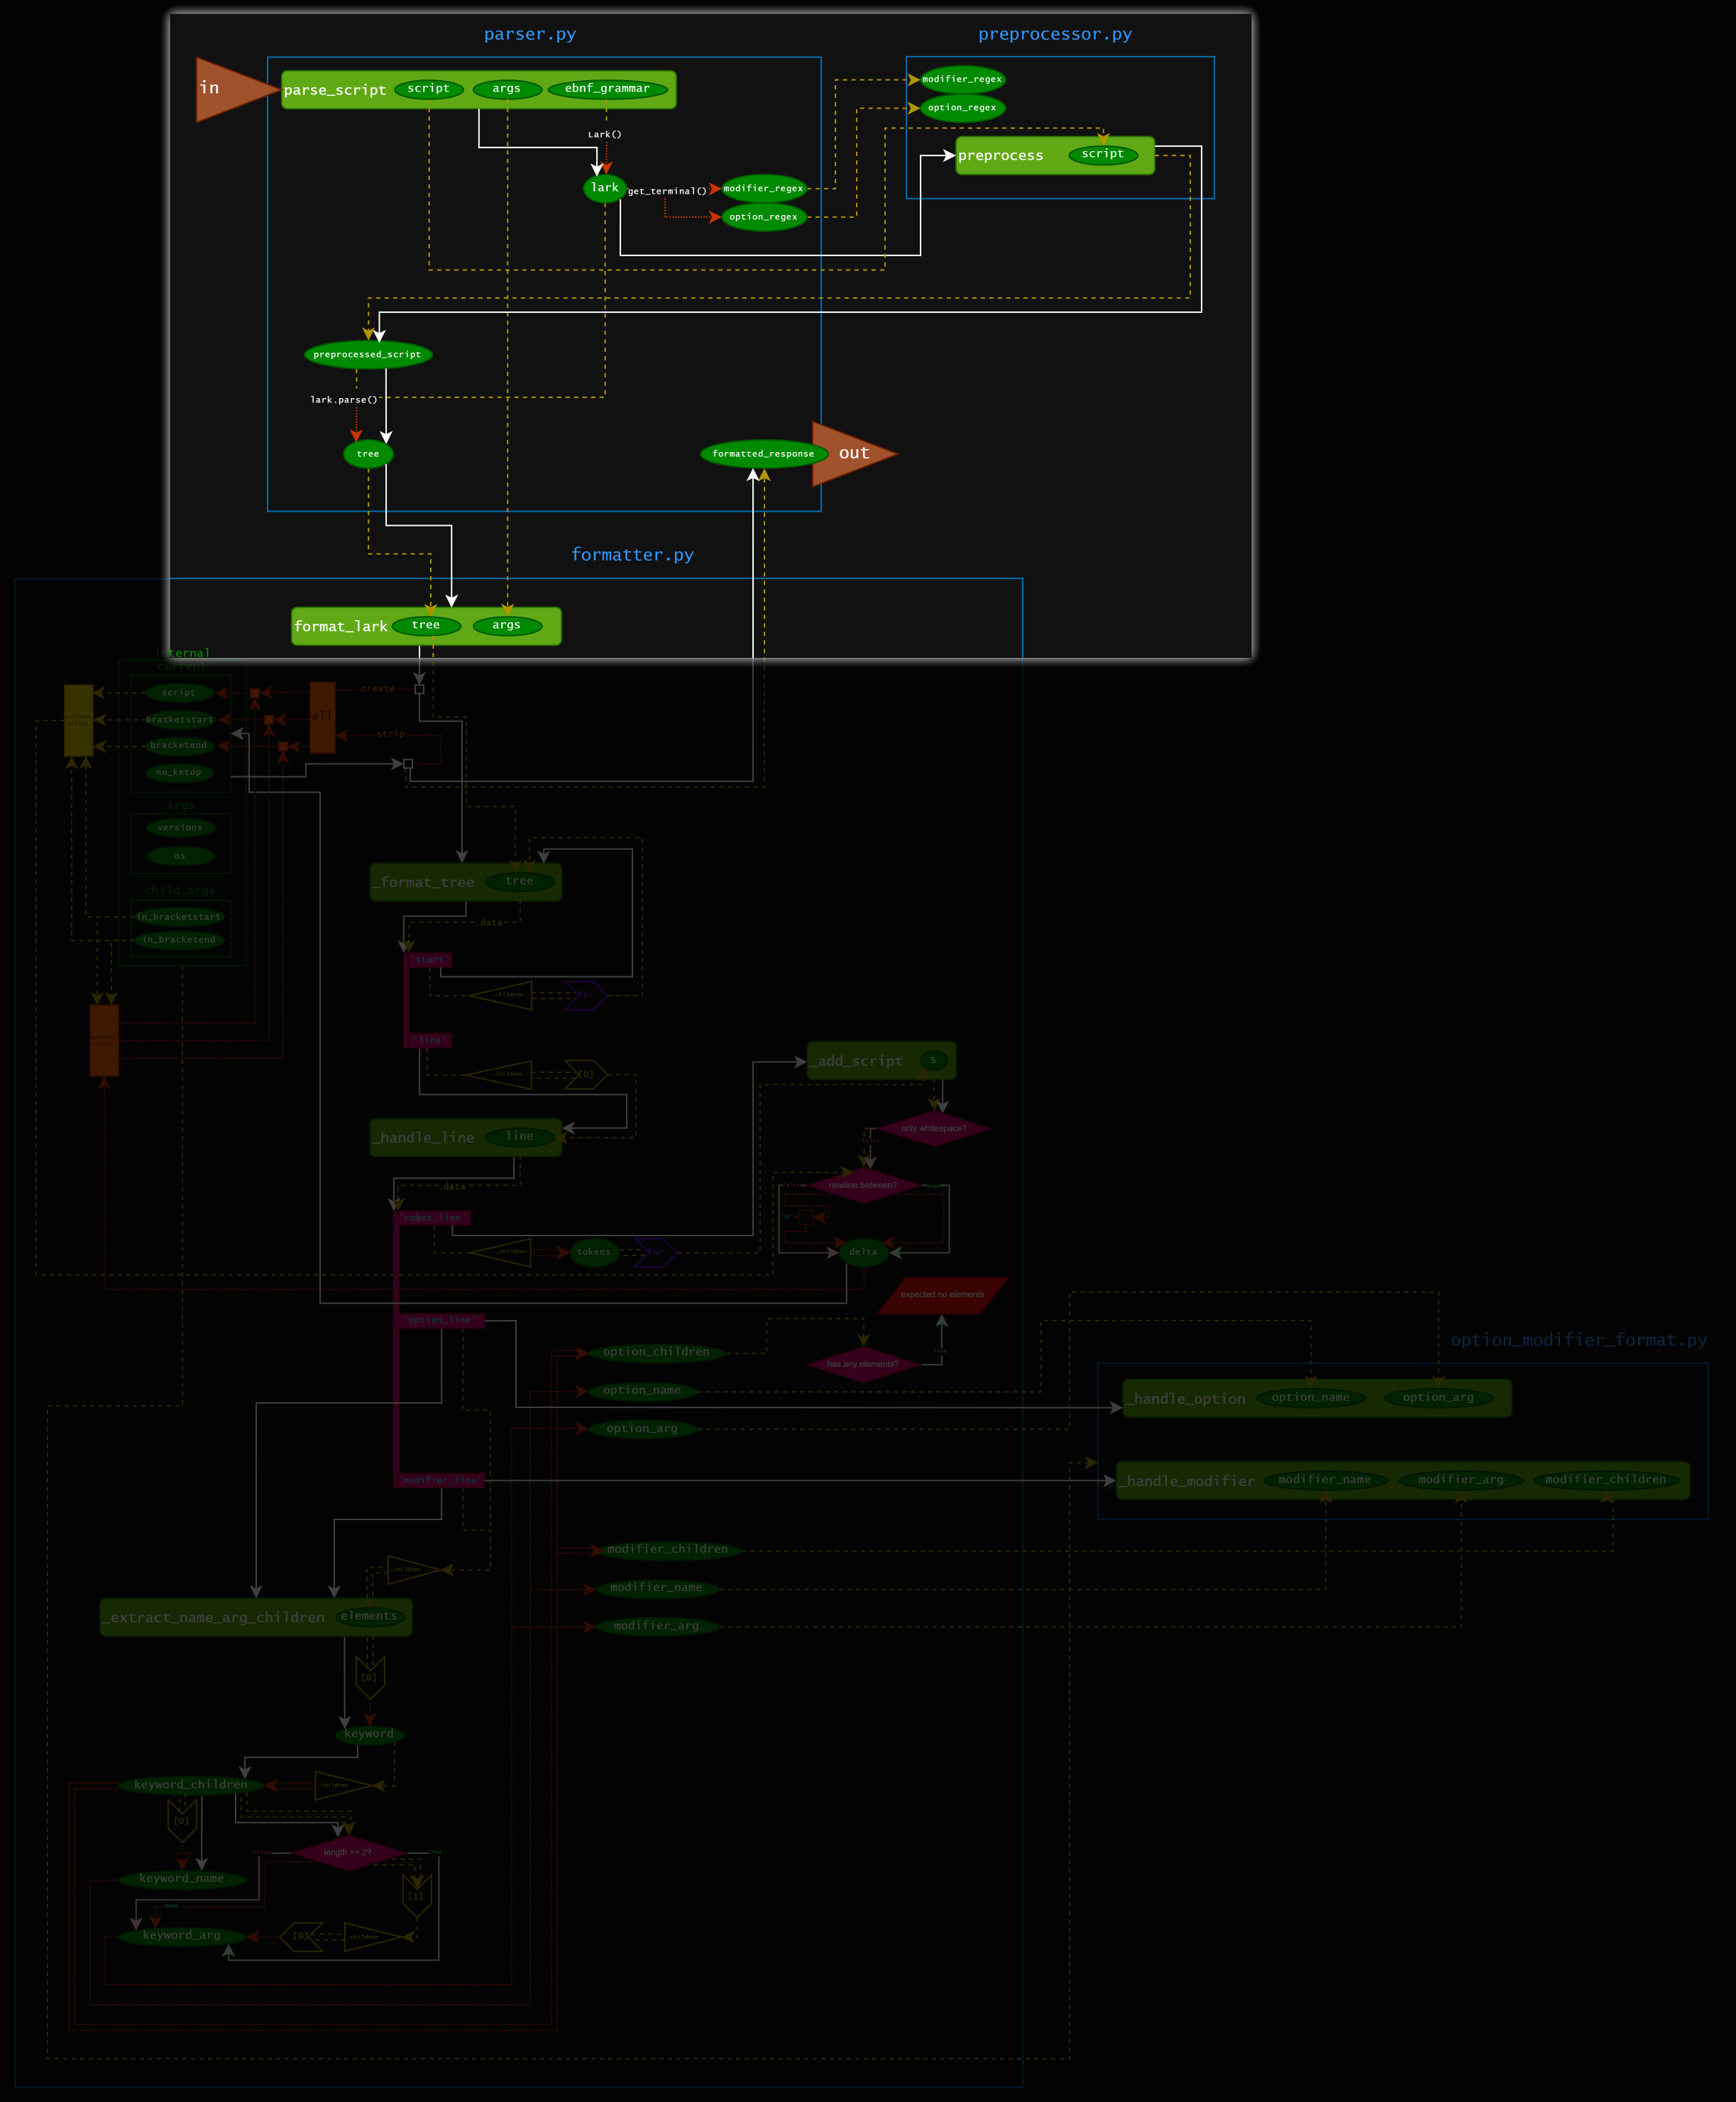
\includegraphics[width=0.35\linewidth]{pics/parser-flowchart/general_location.png}
        \caption{The location of the detailed inset within the full flowchart as seen in Figure~\ref{fig:parser-flowchart_full}.}
        \label{fig:parser-flowchart_general_location}
    \end{subfigure}

    \caption{The part of the flowchart diagram from Figure~\ref{fig:parser-flowchart_full_combined} that details the general procedure of the parser.}
    \label{fig:parser-flowchart_general_combined}
\end{figure}

\section{Formatter}

After a script has been preprocessed and parsed by Lark, the \verb|Tree| object is given to the method from the \verb|Formatter| class with the following header:

\begin{lstlisting}[language=Python, caption={Method header of \texttt{format_lark}.}, label={lst:method_header_parser_format_lark}]
def format_lark(self, tree:Tree, args:FormatterArgs)->FormattedResponse:
\end{lstlisting}

The \verb|Formatter| class recursively parses the \verb|tree|'s children to eventually return a \verb|FormattedResponse|. 

\subsection{FormatterInternal}

The formatter keeps track of the current state of the parsing using an internal property named \verb|current| that is of type \verb|FormatterInternal| which is defined as the following:

\begin{lstlisting}[language=Python, caption={Class definition of \texttt{FormatterInternal}.}, label={lst:class_definition_parser_formatter_internal}]
@dataclass
class FormatterInternal:
    current:FormattedResponse
    args:FormatterArgs
    child_args:ChildArgs
\end{lstlisting}

This \verb|FormatterInternal| instance is unique per formatting operation and it is passed to any functions that need the context of the formatter.\ \verb|args| represents the instance of \verb|FormatterArgs| that was provided to the parser that includes information on versions and operating system. 

When the \verb|format_lark| function finishes without error, it returns the \verb|current| property of the \verb|FormatterInternal| instance it uses to keep track. 

\subsection{ChildArgs}

\verb|child_args| is used for modifiers and their recursive nature. When a line belonging to the block body of a modifier is handled, it may need to be handled differently depending on factors such as whether or not that line should be part of a bracket. 

When a \verb|modifier_line| is hit, the function handling that modifier may return a new instance of \verb|ChildArgs|. Then, this instance will be used for all lines that belong to the block body of that modifier. 

The \verb|ChildArgs| class is defined to be the following:

\begin{lstlisting}[language=Python, caption={Class definition of \texttt{ChildArgs}.}, label={lst:class_definition_parser_child_args}]
@dataclass
class ChildArgs:
    preamble_index:int = 0
    in_bracketstart:bool = False
    in_bracketend:bool = False
\end{lstlisting}

Here, \verb|preamble_index| represents the index of the preamble bracket that new lines should be appended to. If this variable is set to \verb|0|, it means that the formatter is currently not inside of an \verb|@PREAMBLE| modifier. 

\verb|in_bracketstart| and \verb|in_bracketend| represent whether or not the formatter is currently within a respective \verb|@BRACKETSTART| or \verb|@BRACKETEND| modifier. If either of this is the case, new lines will be appended to the respective \verb|bracketstart| or \verb|bracketend| brackets, respectively.

Here, \verb|preamble_index|, \verb|in_bracketstart|, and \verb|in_bracketend| are mutually exclusive to one another, i.e.\ at most only one of them can be \textit{active} at a time.

\subsection{Line handling}

After the formatter is past the \verb|"start"| entry point of the initial \verb|Tree|, it will run \verb|dle_line| on each line element, which is a function with the following header:

\begin{lstlisting}[language=Python, caption={Method header of \texttt{_handle_line}.}, label={lst:method_definition_parser_handle_line`'}]
def _handle_line(self, line:Tree)->None:
\end{lstlisting}

This function differentiates whether the \verb|line| matches \verb|"robot_line"|, \verb|"option_line"|, or \verb|"modifier_line"| in the following way. Note that all functions listed below will be explained shortly. 

\begin{itemize}
    \item For \verb|"robot_line"|: Since Robot lines are made of, for the purposes of the parser, arbitrary text, they can be added to the output as-is using the \verb|_add_script| function.
    \item For \verb|"option_line"|: The function \verb|OptionModifierFormat.handle_option| is called with the current \verb|FormatterInternal|, the option's name (e.g.\ \verb|"NO_KETOP"|), and, if present, the argument string.
    \item For \verb|"modifier_line"|: The function \verb|OptionModifierFormat.handle_modifier| is called with the current \verb|FormatterInternal|, the modifier's name (e.g.\ \verb|"VERSION"|), if present, the argument string (i.e.\ \verb|BIOS > 1.0.0|), and its children. The children represent the modifier line's block body. Then, the output of this function is given to the \verb|_format_children| function for further processing.
\end{itemize}

\verb|_add_script| adds an input string to the output script or respective bracket. This is the function that appends text (Robot lines) to the final \verb|FormattedResponse|. Where exactly the text gets appended to depends on the state of the current \verb|child_args|. If \verb|child_args| specifies that the formatter is currently within a bracket, it will be appended to \verb|bracketstart|, \verb|bracketend|, or the given index of \verb|preamble_dict|, respectively; otherwise, it will be appended to \verb|script|.

\verb|OptionModifierFormat.handle_option| is part of a seperate class to handle the specific option and, in turn, alter flags of the \verb|current| (\verb|FormattedResponse|) provided in the \verb|FormatterInternal| instance. 

\verb|OptionModifierFormat.handle_modifier| is part of a separate class to handle the specific modifier. Unlike \verb|OptionModifierFormat.handle_option|, this function has return values: firstly, its children (which, as stated above, represent the block body) and the new instance of \verb|ChildArgs| to be used as context information for the lines in its block body. 

\verb|_format_children| sets the formatter's current \verb|ChildArgs| to the instance given as parameter, runs \verb|_handle_line| on each element of the provided list of \verb|Tree|s, and then changes the formatter's current \verb|ChildArgs| value back to what it was at the beginning of this function call. This way, a modifier's \verb|ChildArgs| only gets used for its children (block body). If a modifier does not need to pass custom \verb|ChildArgs| to its children, it may return the \verb|ChildArgs| of \verb|current| (\verb|FormatterInternal|), as opposed to a new instance. 

Figures~\ref{fig:parser-flowchart_line-formatting_combined} and~\ref{fig:parser-flowchart_line-formatting_location} highlight the precise procedure to recursively handle each line.

% Ensure floats before are flushed, then place figures at the top
\FloatBarrier
% Combine the two detailed images into one figure and put the location image separately
\begin{figure}[t!]
    \centering
    \begin{subfigure}[b]{\linewidth}
        \centering
        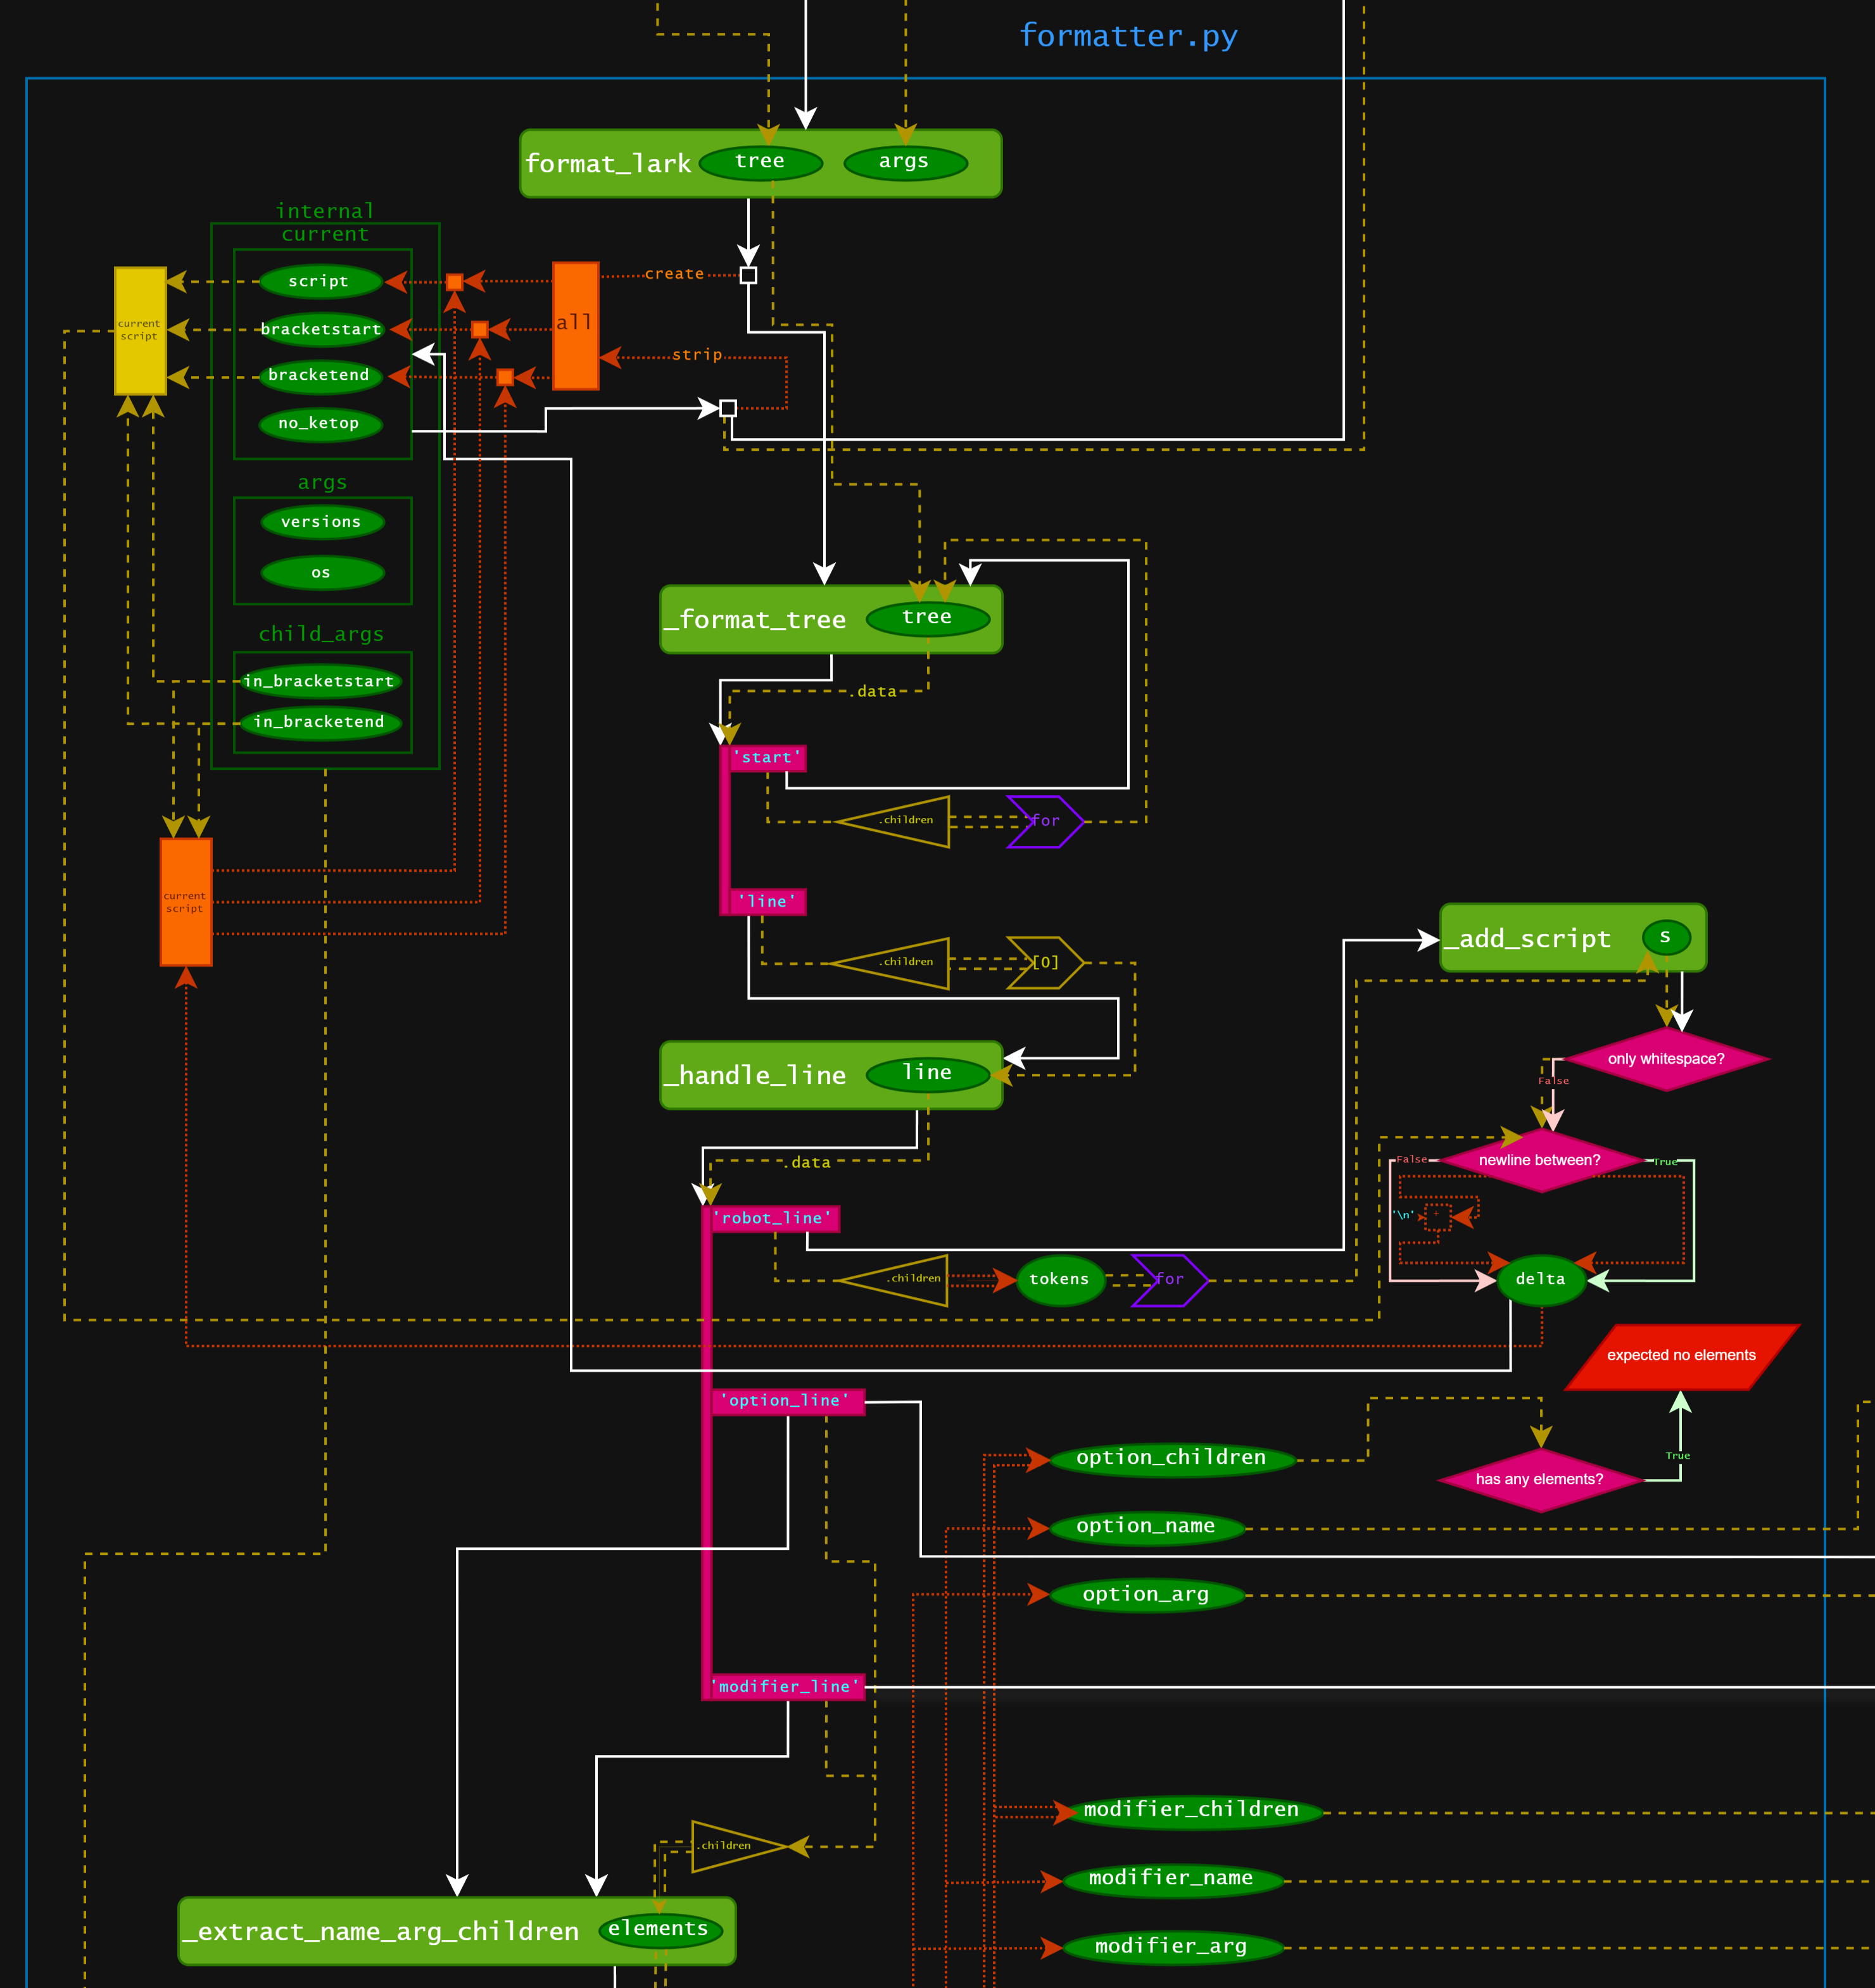
\includegraphics[width=\linewidth]{pics/parser-flowchart/line-formatting-1.png}
        \caption{The detailed part of the parser's flowchart diagram which illustrates how the main part of the formatter recursively handles lines.}
        \label{fig:parser-flowchart_line-formatting-1}
    \end{subfigure}

    \vspace{6pt}

    \begin{subfigure}[b]{\linewidth}
        \centering
        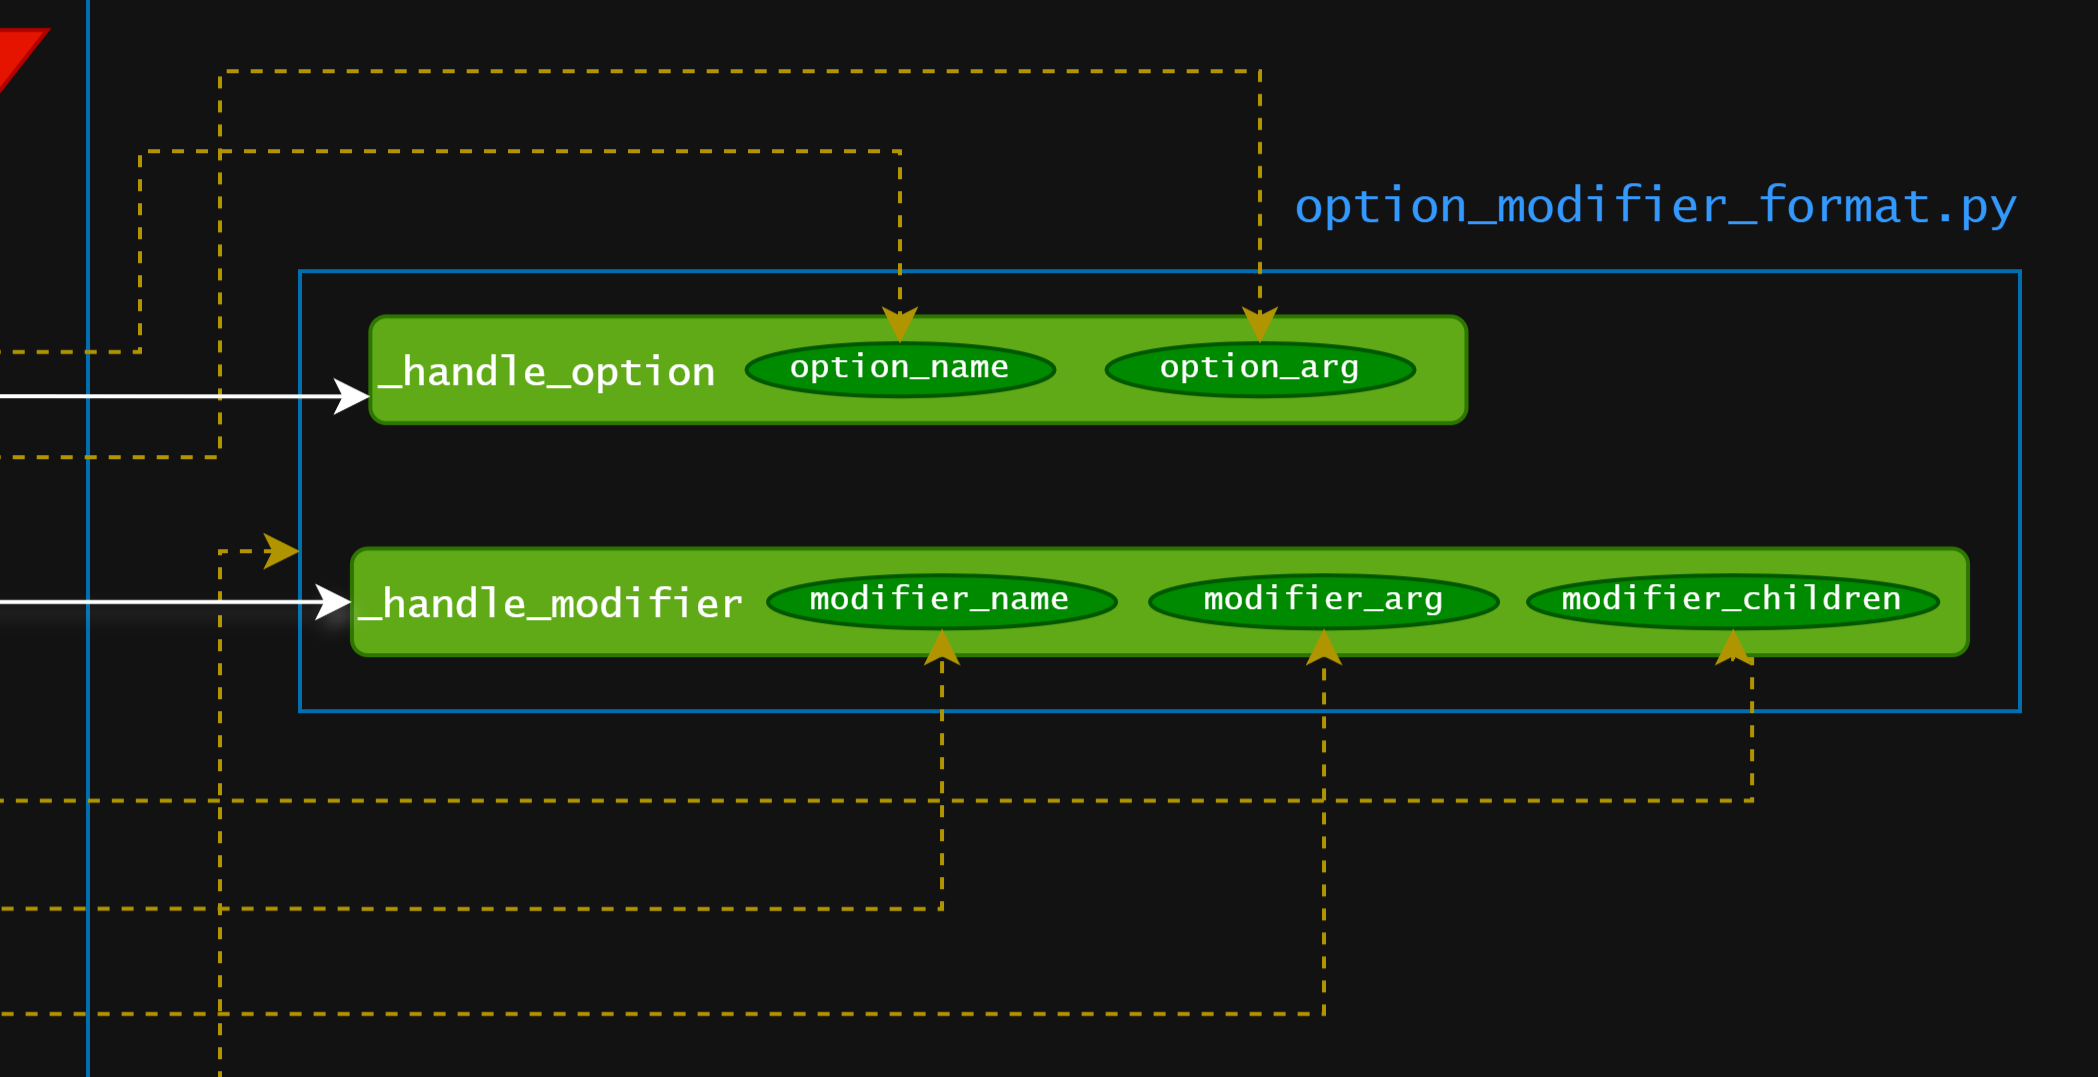
\includegraphics[width=0.7\linewidth]{pics/parser-flowchart/line-formatting-2.png}
        \caption{The detailed part of the parser's flowchart diagram which shows how arguments are passed to Option/Modifier Format.}
        \label{fig:parser-flowchart_line-formatting-2}
    \end{subfigure}

    \caption{Detailed insets for the parser flowchart shown in Figure~\ref{fig:parser-flowchart_full_combined}.}
    \label{fig:parser-flowchart_line-formatting_combined}
\end{figure}

\begin{figure}[t!]
    \centering
    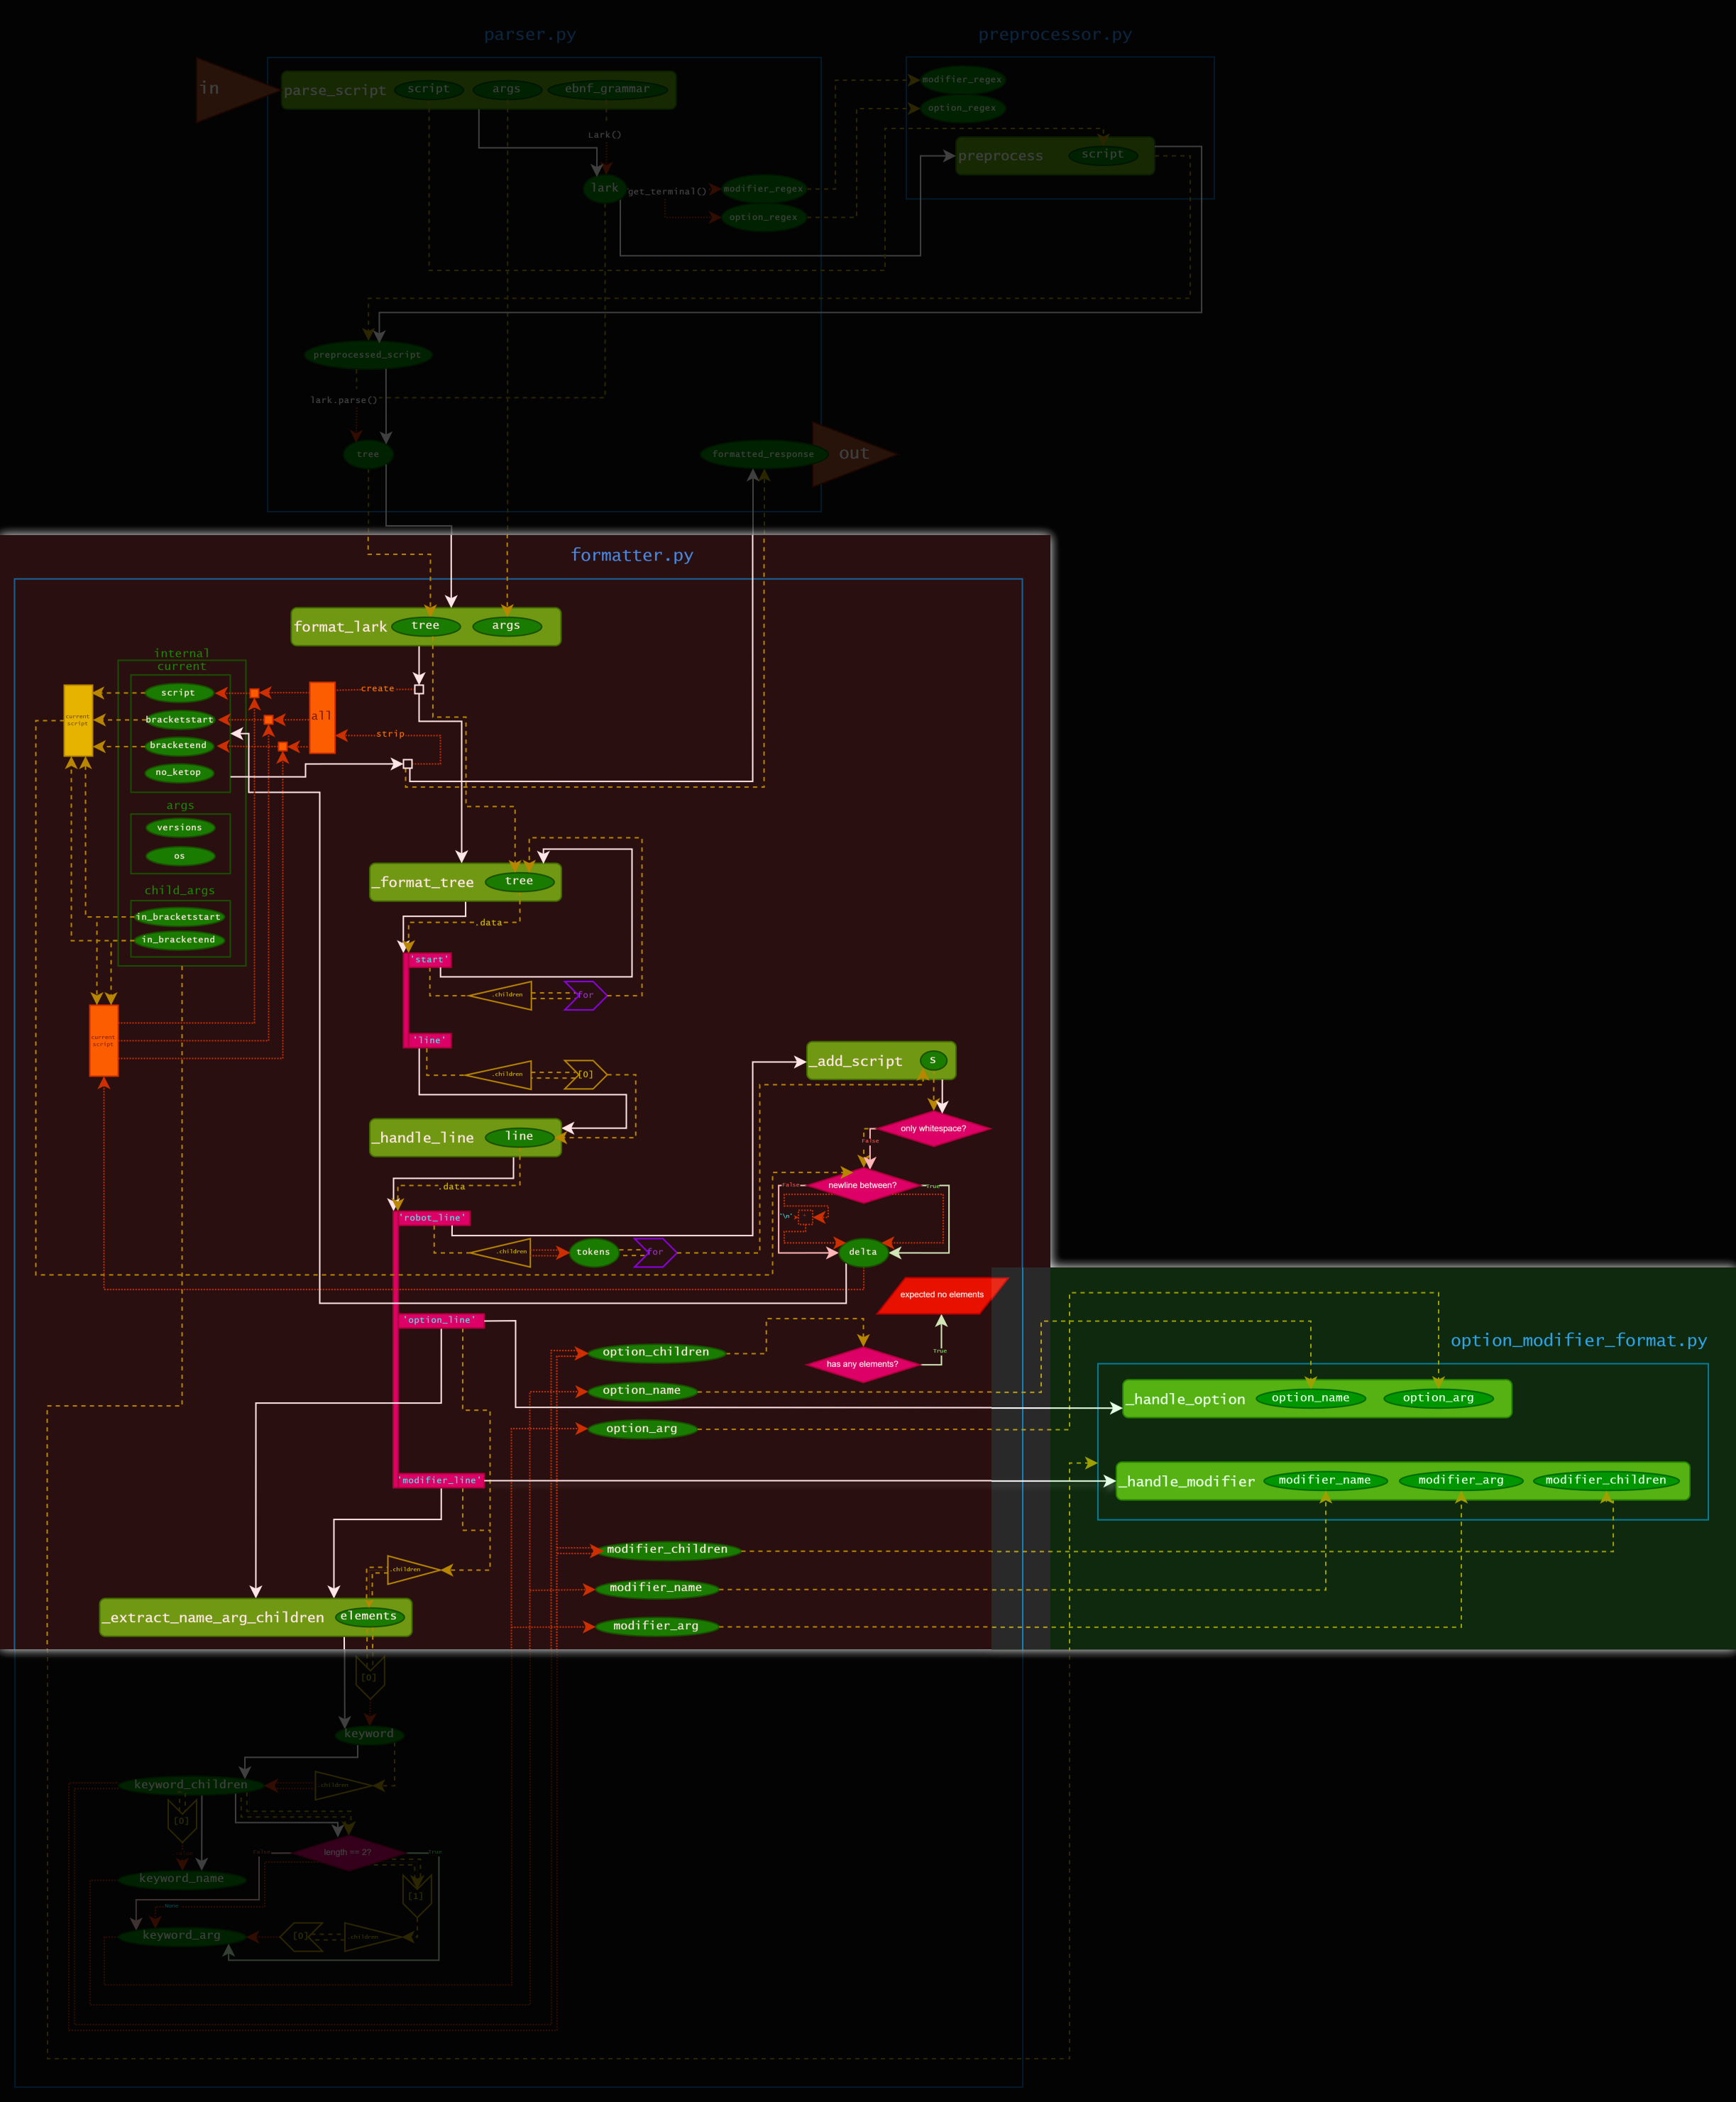
\includegraphics[width=0.45\linewidth]{pics/parser-flowchart/line-formatting_location.png}
    \caption{Location of the detailed insets from Figure~\ref{fig:parser-flowchart_line-formatting_combined} within the full flowchart (Figure~\ref{fig:parser-flowchart_full}).}
    \label{fig:parser-flowchart_line-formatting_location}
\end{figure}

\clearpage

\section{Extracting name, arg, children}

A keyword's name, its argument if present, and its children (block body) get extracted from the \verb|_extract_name_arg_children| function. In the case of an option, the expected amount of children is zero. 

In both cases however, the \verb|children| of the line get passed to this function. Assuming the input to be in the correct general format, the following can be said about the values of the elements of this list, which will be referred to as \verb|elements|:

\begin{itemize}
    \item \verb|elements[0]|: This represents the keyword as option or modifier.\\ 
    Its \verb|$.data| is either \verb|"option"| or \verb|"modifier"|.
    \item \verb|elements[0].children|: This list either contains one or two elements.
    \item \verb|elements[0].children[0]|: This element is a \verb|Token| and its \verb|$.value| represents the name of the keyword (e.g.\ \verb|"VERSION"|). 
    \item \verb|elements[0].children[1]|: If present (i.e.\ if \verb|elements[0].children| contains two elements), its \verb|$.children[0].value| represents the argument. Otherwise, there is no argument. 
    \item \verb|elements[1:]|: The rest of the \verb|elements| list, i.e.\ everything but the first element, is considered the children (block body) of the modifier.
\end{itemize}

Here, \verb|$| is used as a placeholder for the respective variable from before the colon of each bullet point.

Figure~\ref{fig:parser-flowchart_extract-name-arg-children_combined} highlights this procedure.

\begin{figure}[H]
    \centering
    
    \begin{subfigure}[b]{\linewidth}
        \centering
        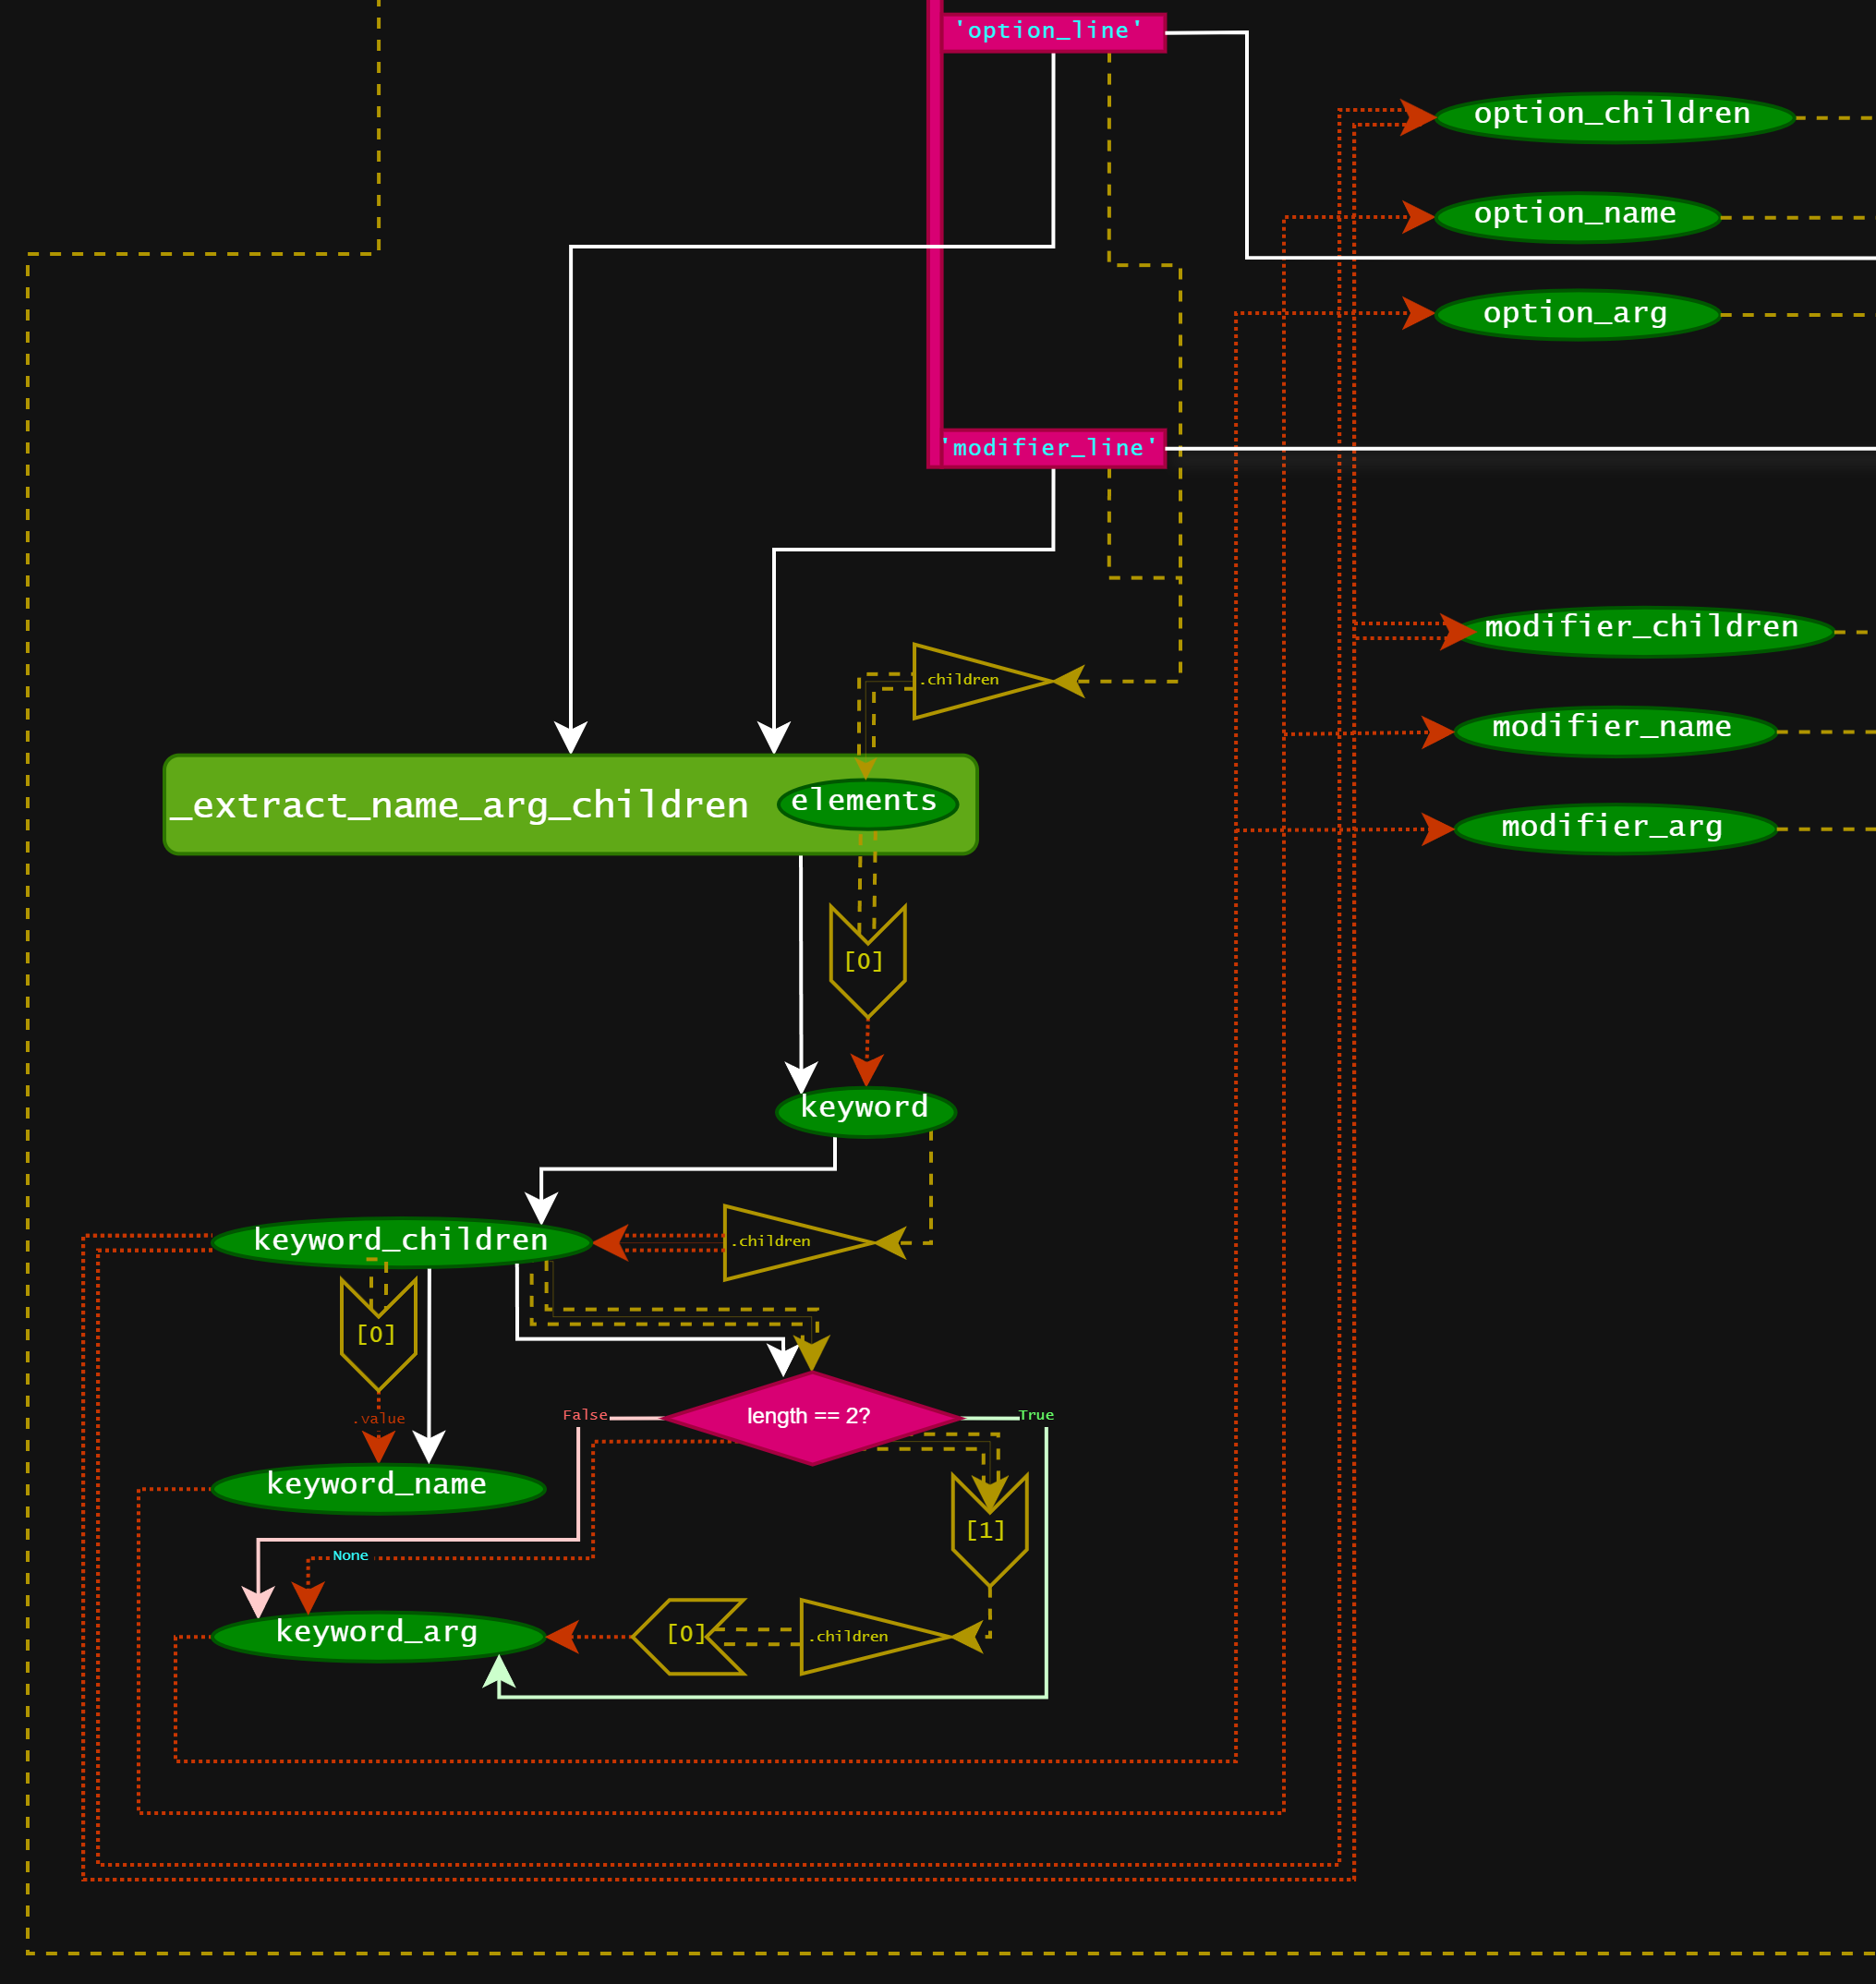
\includegraphics[width=0.8\linewidth]{pics/parser-flowchart/extract-name-arg-children.png}
        \caption{The detailed part of the parser's flowchart diagram which illustrates the extract-name-arg-children procedure.}
        \label{fig:parser-flowchart_extract-name-arg-children}
    \end{subfigure}

    \vspace{6pt}

    \begin{subfigure}[b]{\linewidth}
        \centering
        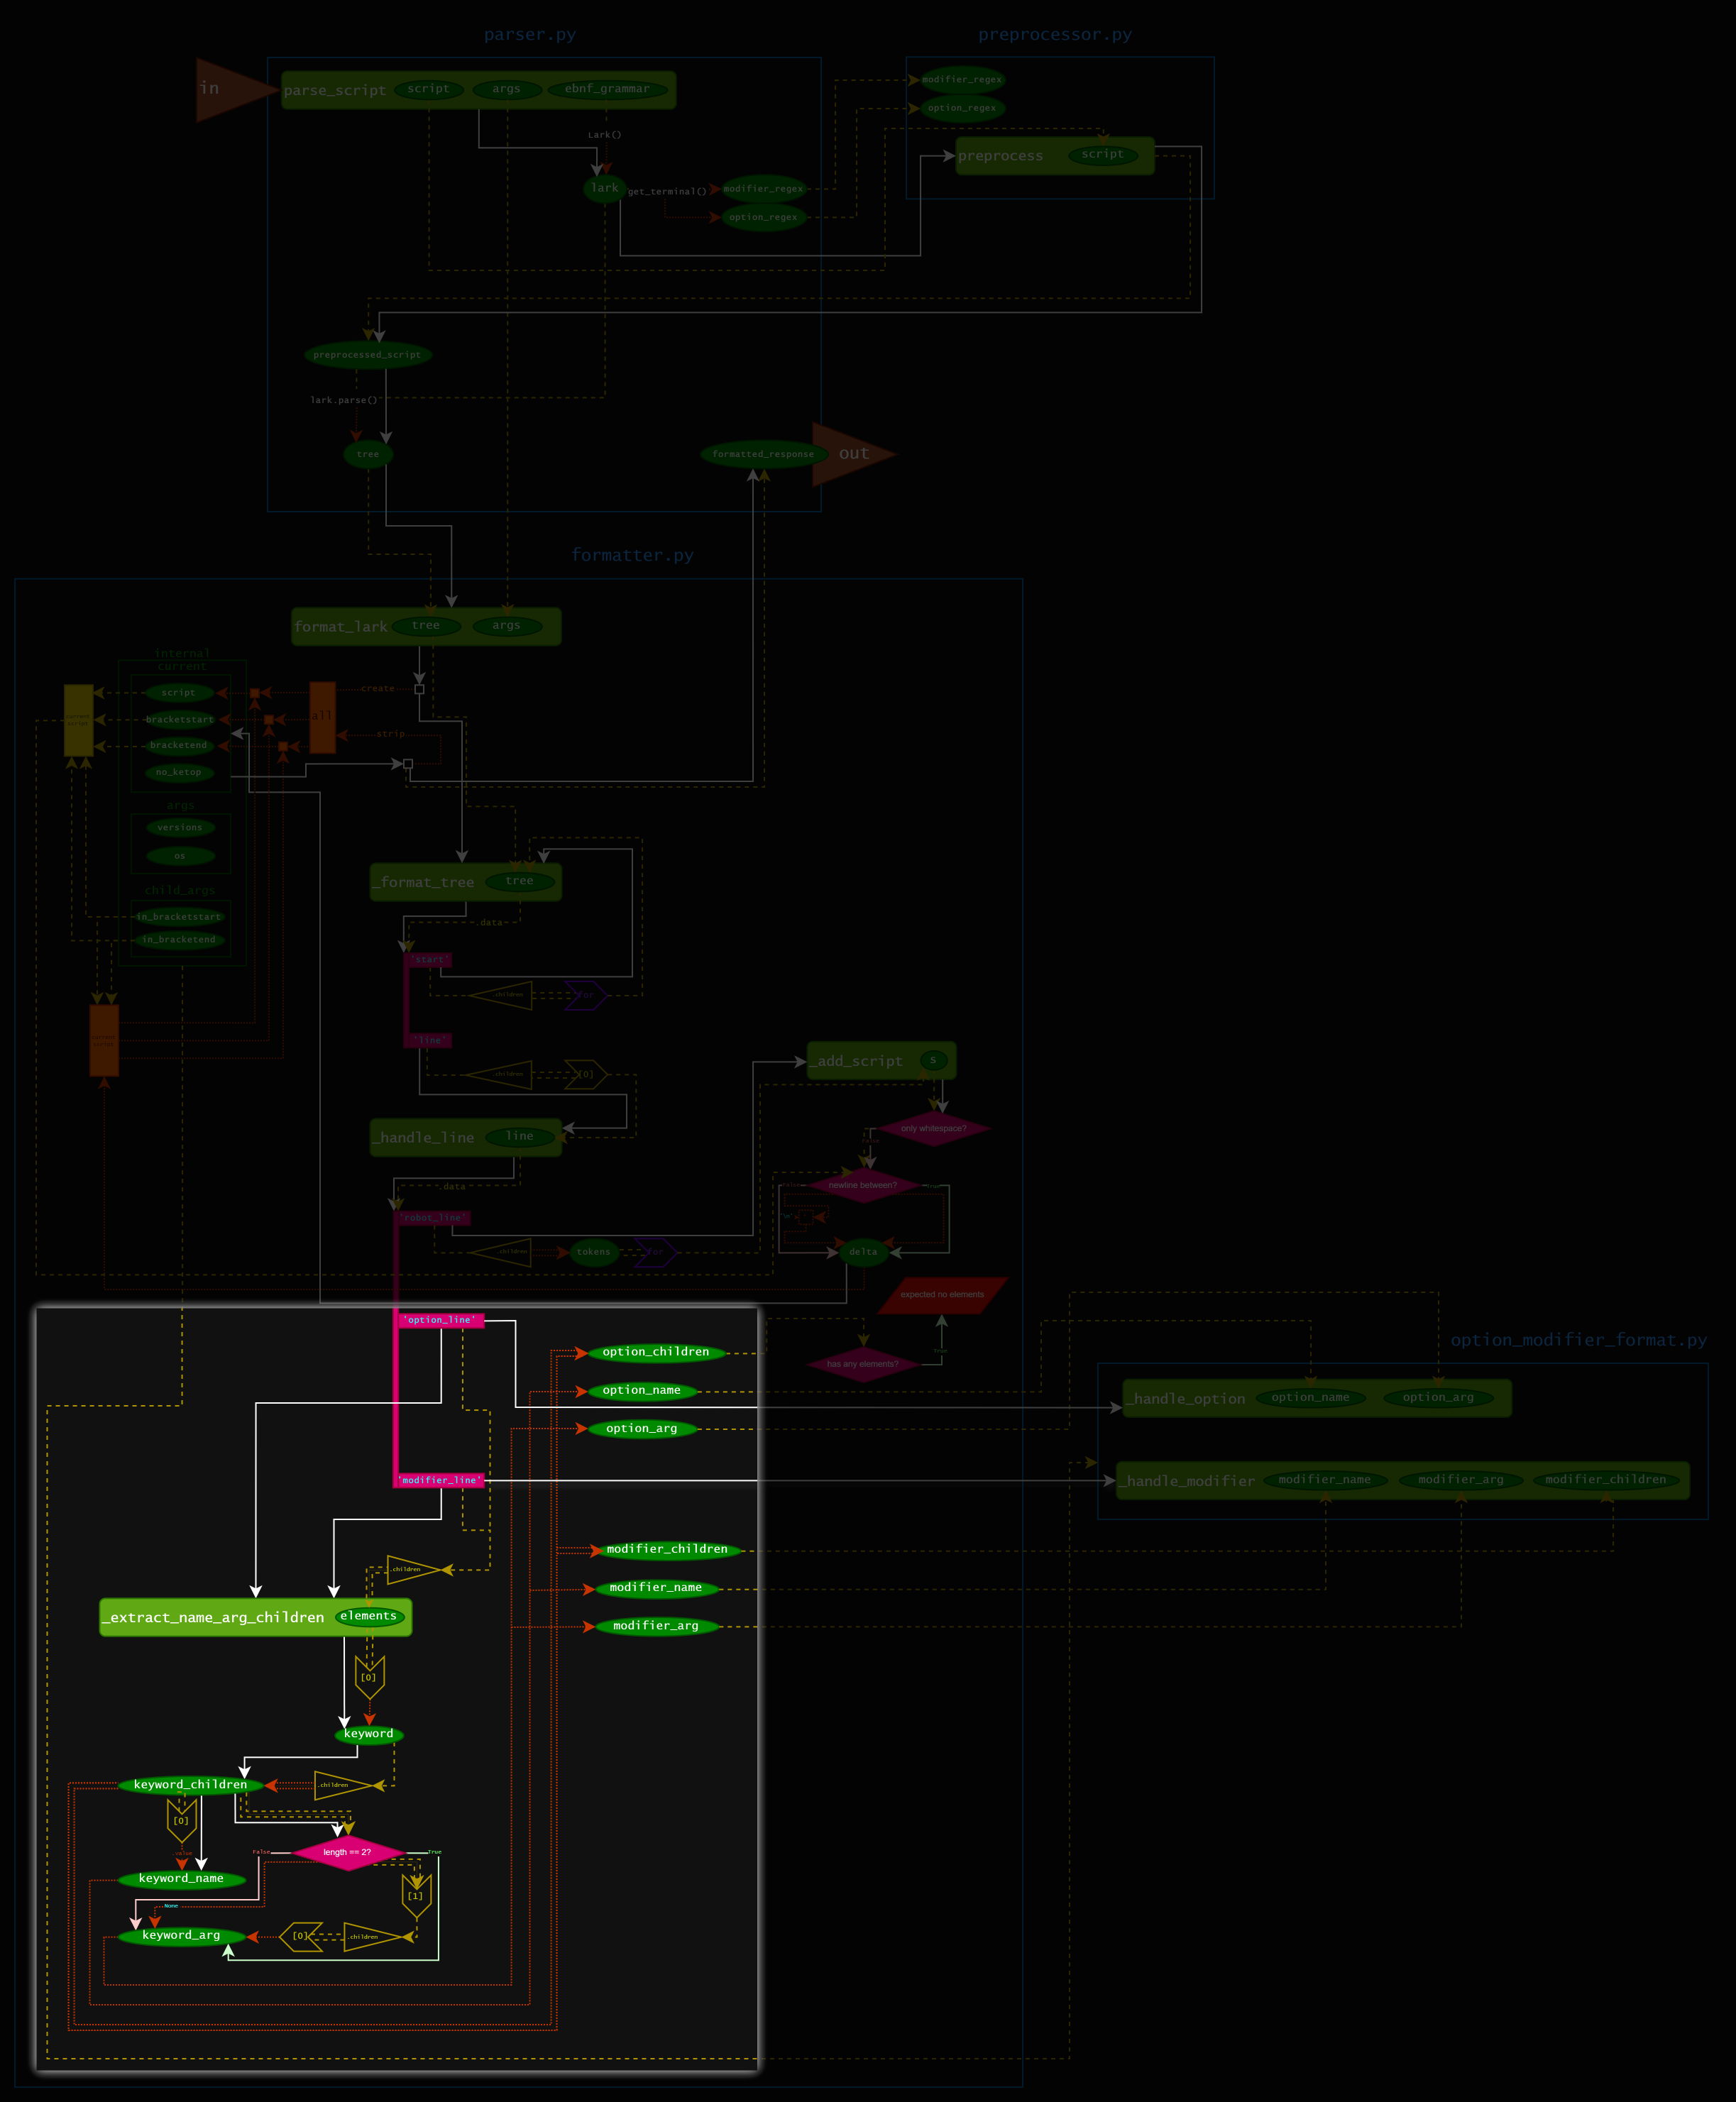
\includegraphics[width=0.35\linewidth]{pics/parser-flowchart/extract-name-arg-children_location.png}
        \caption{The location of the detailed inset within the full flowchart as seen in Figure~\ref{fig:parser-flowchart_full}.}
        \label{fig:parser-flowchart_extract-name-arg-children_location}
    \end{subfigure}

    \caption{The part of the flowchart diagram from Figure~\ref{fig:parser-flowchart_full_combined} that details the extract-name-arg-children procedure of the parser.}
    \label{fig:parser-flowchart_extract-name-arg-children_combined}
\end{figure}

